\documentclass[10pt, aspectratio=43,compress]{beamer}
\usepackage[utf8]{inputenc}
\usepackage[T1]{fontenc}
\usepackage{lmodern}
\usepackage{tcolorbox}
\usepackage{amsmath}
\usepackage{amsfonts}
\usepackage{amssymb}
\usepackage{amsthm}
\usepackage{stmaryrd}
\usepackage{caption}
\usepackage{appendixnumberbeamer}

\usepackage{algorithm,algpseudocode}
\usepackage{cancel}

\usepackage{adjustbox}

\usepackage[document]{ragged2e}
\makeatletter
\DeclareOldFontCommand{\rm}{\normalfont\rmfamily}{\mathrm}
\DeclareOldFontCommand{\sf}{\normalfont\sffamily}{\mathsf}
\DeclareOldFontCommand{\tt}{\normalfont\ttfamily}{\mathtt}
\DeclareOldFontCommand{\bf}{\normalfont\bfseries}{\mathbf}
\DeclareOldFontCommand{\it}{\normalfont\itshape}{\mathit}
\DeclareOldFontCommand{\sl}{\normalfont\slshape}{\@nomath\sl}
\DeclareOldFontCommand{\sc}{\normalfont\scshape}{\@nomath\sc}
\makeatother

% \beamerdefaultoverlayspecification{<+->}

\newcommand{\X}{\mathsf{X}}
\newcommand{\Y}{\mathsf{Y}}
\renewcommand{\S}{\mathcal{S}}
\newcommand{\T}{\mathcal{T}}


\newcommand{\defeq}{\overset{\textsf{def}}{=}}

\usepackage{datetime}
\usepackage{nameref}

\usepackage{tikz}
\usepackage{pgfplots}

\usepackage{enumerate}
\usepackage{tikz}
\usetikzlibrary{decorations.pathreplacing}
\usetikzlibrary{patterns}
\usetikzlibrary{patterns.meta}
\usetikzlibrary{calc}

\usepackage{float}
\usepackage{multicol}

\definecolor{magenta}{rgb}{1.0, 0.0, 1.0}
\definecolor{alizarin}{rgb}{0.82, 0.1, 0.26}
\definecolor{antiquebrass}{rgb}{0.8, 0.58, 0.46}
\definecolor{darkturquoise}{rgb}{0.0, 0.81, 0.82}
\definecolor{darkpastelgreen}{rgb}{0.01, 0.75, 0.24}
\definecolor{darktangerine}{rgb}{1.0, 0.66, 0.07}
\definecolor{richcarmine}{rgb}{0.84, 0.0, 0.25}
\definecolor{majorelleblue}{rgb}{0.38, 0.31, 0.86}
\definecolor{magenta}{rgb}{1.0, 0.0, 1.0}
\definecolor{cobalt}{rgb}{0.0, 0.28, 0.67}
\definecolor{ferrarired}{rgb}{1.0, 0.11, 0.0}
\definecolor{battleshipgrey}{rgb}{0.52, 0.52, 0.51}
\definecolor{atomictangerine}{rgb}{1.0, 0.6, 0.4}
\definecolor{caribbeangreen}{rgb}{0.0, 0.8, 0.6}
\definecolor{lightsalmon}{rgb}{1.0, 0.63, 0.48}
\definecolor{darkseagreen}{rgb}{0.56, 0.74, 0.56}

% \usetheme{Bergen}
% \usetheme{Berlin}
% \usetheme{classic}
% \usetheme{Darmstadt}
% \usetheme{Dresden}
\usetheme{EastLansing}
% \usetheme{Frankfurt}

\setbeamertemplate{section in toc}[square]

\definecolor{cadmiumgreen}{rgb}{0.0, 0.42, 0.24}
\definecolor{airforceblue}{rgb}{0.36, 0.54, 0.66}
\definecolor{bondiblue}{rgb}{0.0, 0.58, 0.71}

\newtheorem*{conj*}{Conjecture}
\newtheorem*{lmm*}{Lemme}

% \setbeamercovered{transparent}
\makeatother
\author{Benoît \textsc{Bompol}, Armand \textsc{Grenier}}
\subtitle{Combinatorial Optimization and Graph Theory}
\title[Directed hypergraph connectivity augmentation]{\textsf{\textbf{Directed hypergraph connectivity augmentation by hyperarc re-orientations}}}
\date{Thursday, Nov 23rd 2023}

\pgfplotsset{compat=1.18}
\begin{document}
	\begin{frame}[plain]
		\maketitle
	\end{frame}
	
	\begin{frame}{Table of contents}
		\tableofcontents
	\end{frame}
	
	\section{Introduction}
	\begin{frame}{State of the art, goal of the article}
		\visible<1->{
			\begin{tcolorbox}[colback=richcarmine!5!white,colframe=richcarmine!75!black,title=Nash-Williams (1960)]
				$G$ is a $2k$-edge connected undirected graph $\Leftrightarrow$ $G$ admits a $k$-arc connected orientation.
			\end{tcolorbox}
		}
		
		\visible<2->{
			\begin{tcolorbox}[colback=richcarmine!5!white,colframe=richcarmine!75!black,title=Ito et al (2023)]
				\begin{itemize}
					\item Algorithmic proof of \textit{Nash-Williams}, by flipping one arc at a time.
					\item Exhibiting a sequence of orientations such that :
						\begin{itemize}
							\item The arc-connectivity does not decrease, and the arc-connectivity of the last element of the sequence is $k$.
							\item The next orientation in the sequence can be obtained from the previous one by flipping exactly one arc.
							\item The sequence can be obtained in polynomial time (in the size of the directed graph).
						\end{itemize}	
				\end{itemize}
			\end{tcolorbox}
		}
		
		\visible<3->{Goal of the article : Expanding the result of \textbf{Ito and al.} to hypergraphs.}
	\end{frame}
	
	\begin{frame}{Hypergraphs}    
		\begin{figure}[H]
			\centering
			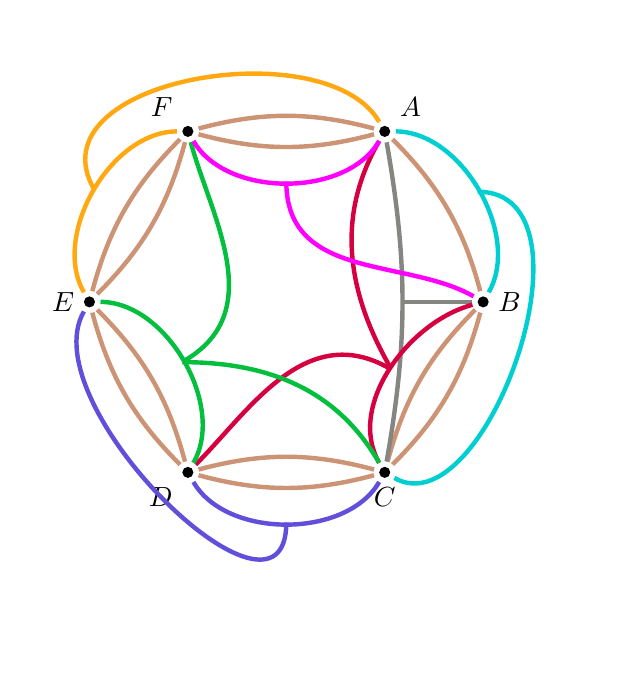
\begin{tikzpicture}
				\def\radius{2.5}
				\coordinate (A) at (60:\radius);
				\coordinate (B) at (0:\radius);
				\coordinate (C) at (300:\radius);
				\coordinate (D) at (240:\radius);
				\coordinate (E) at (180:\radius);
				\coordinate (F) at (120:\radius);
				
				\fill (A) circle (2pt); \node[above right=2pt] at (A) {$A$};
				\fill (B) circle (2pt); \node[right=2pt] at (B) {$B$};
				\fill (C) circle (2pt); \node[below=2pt] at (C) {$C$};
				\fill (D) circle (2pt); \node[below left=2pt] at (D) {$D$};
				\fill (E) circle (2pt); \node[left=2pt] at (E) {$E$};
				\fill (F) circle (2pt); \node[above left=2pt] at (F) {$F$};
				
				\visible<3>{
					\draw[ultra thick, antiquebrass, shorten <= 4pt, shorten >= 4pt] (E) to [out=75, in=-135] (F);
				}
				
				\visible<4->{
					\draw[ultra thick, antiquebrass, shorten <= 4pt, shorten >= 4pt] (A) to [out=-45, in=105] (B);
					\draw[ultra thick, antiquebrass, shorten <= 4pt, shorten >= 4pt] (B) to [out=-105, in=45] (C);
					\draw[ultra thick, antiquebrass, shorten <= 4pt, shorten >= 4pt] (C) to [out=195, in=-15] (D);
					\draw[ultra thick, antiquebrass, shorten <= 4pt, shorten >= 4pt] (D) to [out=135, in=-75] (E);
					\draw[ultra thick, antiquebrass, shorten <= 4pt, shorten >= 4pt] (F) to [out=15, in=165] (A);
				}
				
				\visible<4->{
					\draw[ultra thick, antiquebrass, shorten <= 4pt, shorten >= 4pt] (A) to [out=195, in=-15] (F);            \draw[ultra thick, antiquebrass, shorten <= 4pt, shorten >=4pt] (C) to [out=75, in=-135] (B);
					\draw[ultra thick, antiquebrass, shorten <= 4pt, shorten >= 4pt] (D) to [out=15, in=165] (C);
					\draw[ultra thick, antiquebrass, shorten <= 4pt, shorten >= 4pt] (E) to [out=-45, in=105] (D);
					\draw[ultra thick, antiquebrass, shorten <= 4pt, shorten >= 4pt] (F) to [out=-105, in=45] (E);
				}
				
				\visible<2->{
					% {AC -> B}
					\draw[ultra thick, battleshipgrey, shorten <= 4pt, shorten >= 4pt] (A) to [out=-80, in=80] node[pos=0.5] (ac) {} (C);
					\draw[ultra thick, battleshipgrey, shorten <= -4pt, shorten >= 4pt] (ac) to [out = 0, in = 180] (B);
				}
				
				
				\visible<4->{
					% {AB -> C}
					\draw[ultra thick, darkturquoise, shorten <= 4pt, shorten >= 4pt] (A) to [out=0, in=60] node[pos=0.5] (ab) {}   (B);
					\draw[ultra thick, darkturquoise, shorten <= -4pt, shorten >= 4pt] (ab) to [out = 0, in = -30] (C);
				}
				
				\visible<4->{
					% {ABC -> D}
					\draw[ultra thick, richcarmine, shorten <= 4pt, shorten >= 4pt] (B) to [out=195, in=120] node[pos=0.5] (bc) {} (C);
					\draw[ultra thick, richcarmine, shorten <= 4pt, shorten >= -4pt] (A) to [out=-120, in=120] (bc);
					\draw[ultra thick, richcarmine, shorten <= -4pt, shorten >= 4pt] (bc) to [out = 150, in = 45] (D);
				}
				
				\visible<4->{
					% {CD -> E}
					\draw[ultra thick, majorelleblue, shorten <= 4pt, shorten >= 4pt] (C) to [out=240, in=-60] node[pos=0.5] (cd) {} (D);
					\draw[ultra thick, majorelleblue, shorten <= -4pt, shorten >= 4pt] (cd) to [out = -90, in = -120] (E);
				}
				
				\visible<4->{
					% {CDE -> F}
					\draw[ultra thick, darkpastelgreen, shorten <= 4pt, shorten >= 4pt] (D) to [out=60, in=0] node[pos=0.5] (de) {}     (E);
					\draw[ultra thick, darkpastelgreen, shorten <= 4pt, shorten >= -4pt] (C) to [out=120, in=0] (de);
					\draw[ultra thick, darkpastelgreen, shorten <= -4pt, shorten >= 4pt] (de) to [out = 30, in = -75] (F);
				}
				
				\visible<4->{
					% {EF -> A}
					\draw[ultra thick, darktangerine, shorten <= 4pt, shorten >= 4pt] (E) to [out=120,in=180] node[pos=0.5] (ef) {} (F);
					\draw[ultra thick, darktangerine, shorten <= -4pt, shorten >= 4pt] (ef) to [out = 120, in = 120] (A);
				}
				
				\visible<4->{
					% {FA -> B}
					\draw[ultra thick, magenta, shorten <= 4pt, shorten >= 4pt] (F) to [out = -60, in = -120] node[pos=0.5] (fa) {}     (A);
					\draw[ultra thick, magenta, shorten <= -4pt, shorten >= 4pt] (fa) to [out = -90, in = 150] (B);
				}
			\end{tikzpicture}
		\end{figure}
	\end{frame}
	
	\begin{frame}{Degree of $\varnothing\not=\mathsf{X}\subsetneq V$}
		$d_{\mathcal{H}}(\mathsf{X})$ is the number of hyperedges intersecting both $\mathsf{X}$ and $V\setminus\mathsf{X}$.
		\begin{figure}[H]
			\centering
			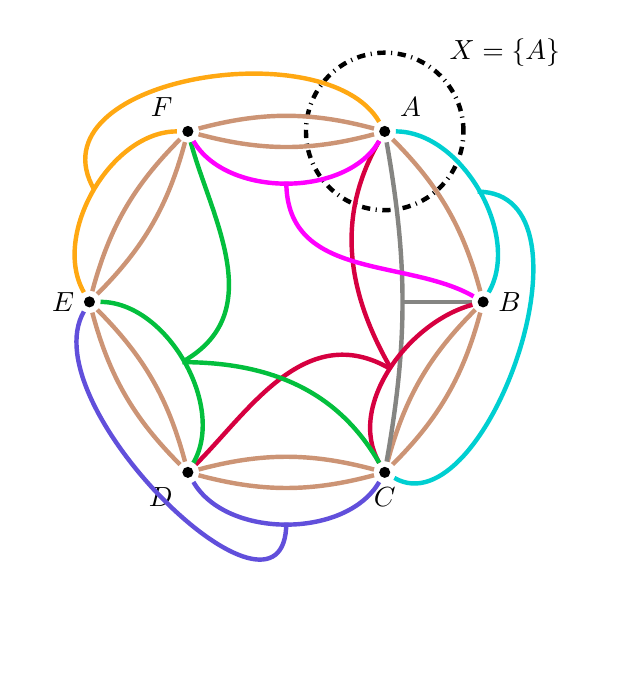
\begin{tikzpicture}
				\def\radius{2.5}
				\coordinate (A) at (60:\radius);
				\coordinate (B) at (0:\radius);
				\coordinate (C) at (300:\radius);
				\coordinate (D) at (240:\radius);
				\coordinate (E) at (180:\radius);
				\coordinate (F) at (120:\radius);
				
				\node[above right=2pt] at (A) {$A$}; \fill (A) circle (2pt);
				\visible<2->{\draw[dashdotted, ultra thick] (A) circle (1); \node[above right=7mm] at (A) {$X=\{A\}$};}
				\fill (B) circle (2pt); \node[right=2pt] at (B) {$B$};
				\fill (C) circle (2pt); \node[below=2pt] at (C) {$C$};
				\fill (D) circle (2pt); \node[below left=2pt] at (D) {$D$};
				\fill (E) circle (2pt); \node[left=2pt] at (E) {$E$};
				\fill (F) circle (2pt); \node[above left=2pt] at (F) {$F$};
				
				
				\visible<-2>{
					\draw[ultra thick, antiquebrass, shorten <= 4pt, shorten >= 4pt] (C) to [out=195, in=-15] (D);
					\draw[ultra thick, antiquebrass, shorten <= 4pt, shorten >= 4pt] (B) to [out=-105, in=45] (C);
					\draw[ultra thick, antiquebrass, shorten <= 4pt, shorten >= 4pt] (D) to [out=135, in=-75] (E);
					\draw[ultra thick, antiquebrass, shorten <= 4pt, shorten >= 4pt] (E) to [out=75, in=-135] (F);
					\draw[ultra thick, antiquebrass, shorten <= 4pt, shorten >=4pt] (C) to [out=75, in=-135] (B);
					\draw[ultra thick, antiquebrass, shorten <= 4pt, shorten >= 4pt] (D) to [out=15, in=165] (C);
					\draw[ultra thick, antiquebrass, shorten <= 4pt, shorten >= 4pt] (E) to [out=-45, in=105] (D);
					\draw[ultra thick, antiquebrass, shorten <= 4pt, shorten >= 4pt] (F) to [out=-105, in=45] (E);
				}
				
				\visible<-3>{
					\draw[ultra thick, antiquebrass, shorten <= 4pt, shorten >= 4pt] (A) to [out=-45, in=105] (B);
					\draw[ultra thick, antiquebrass, shorten <= 4pt, shorten >= 4pt] (A) to [out=195, in=-15] (F);
					\draw[ultra thick, antiquebrass, shorten <= 4pt, shorten >= 4pt] (F) to [out=15, in=165] (A);
				}
				
				\visible<-3>{
					% {AC -> B}
					\draw[ultra thick, battleshipgrey, shorten <= 4pt, shorten >= 4pt] (A) to [out=-80, in=80] node[pos=0.5] (ac) {} (C);
					\draw[ultra thick, battleshipgrey, shorten <= -4pt, shorten >= 4pt] (ac) to [out = 0, in = 180] (B);
					
					% {AB -> C}
					\draw[ultra thick, darkturquoise, shorten <= 4pt, shorten >= 4pt] (A) to [out=0, in=60] node[pos=0.5] (ab) {} (B);
					\draw[ultra thick, darkturquoise, shorten <= -4pt, shorten >= 4pt] (ab) to [out = 0, in = -30] (C);
					
					% {ABC -> D}
					\draw[ultra thick, richcarmine, shorten <= 4pt, shorten >= 4pt] (B) to [out=195, in=120] node[pos=0.5] (bc) {} (C);
					\draw[ultra thick, richcarmine, shorten <= 4pt, shorten >= -4pt] (A) to [out=-120, in=120] (bc);
					\draw[ultra thick, richcarmine, shorten <= -4pt, shorten >= 4pt] (bc) to [out = 150, in = 45] (D);
				}
				
				\visible<-2>{
					% {CD -> E}
					\draw[ultra thick, majorelleblue, shorten <= 4pt, shorten >= 4pt] (C) to [out=240, in=-60] node[pos=0.5] (cd) {} (D);
					\draw[ultra thick, majorelleblue, shorten <= -4pt, shorten >= 4pt] (cd) to [out = -90, in = -120] (E);
					
					% {CDE -> F}
					\draw[ultra thick, darkpastelgreen, shorten <= 4pt, shorten >= 4pt] (D) to [out=60, in=0] node[pos=0.5] (de) {} (E);
					\draw[ultra thick, darkpastelgreen, shorten <= 4pt, shorten >= -4pt] (C) to [out=120, in=0] (de);
					
					\draw[ultra thick, darkpastelgreen, shorten <= -4pt, shorten >= 4pt] (de) to [out = 30, in = -75] (F);
				}
				
				\visible<-3>{
					% {EF -> A}
					\draw[ultra thick, darktangerine, shorten <= 4pt, shorten >= 4pt] (E) to [out=120,in=180] node[pos=0.5] (ef) {} (F);
					\draw[ultra thick, darktangerine, shorten <= -4pt, shorten >= 4pt] (ef) to [out = 120, in = 120] (A);
					
					% {FA -> B}
					\draw[ultra thick, magenta, shorten <= 4pt, shorten >= 4pt] (F) to [out = -60, in = -120] node[pos=0.5] (fa) {}  (A);
					\draw[ultra thick, magenta, shorten <= -4pt, shorten >= 4pt] (fa) to [out = -90, in = 150] (B);
				}
				
			\end{tikzpicture}
		\end{figure}
	\end{frame}
	
	\begin{frame}{Orientation of an hypergraph}
		\begin{figure}[H]
			\centering
			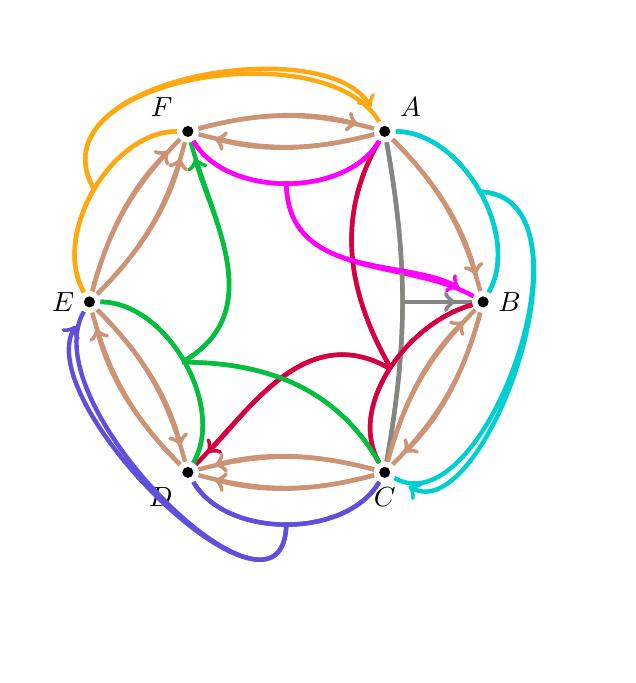
\begin{tikzpicture}
				\def\radius{2.5}
				\coordinate (A) at (60:\radius);
				\coordinate (B) at (0:\radius);
				\coordinate (C) at (300:\radius);
				\coordinate (D) at (240:\radius);
				\coordinate (E) at (180:\radius);
				\coordinate (F) at (120:\radius);
				
				\fill (A) circle (2pt); \node[above right=2pt] at (A) {$A$};
				\fill (B) circle (2pt); \node[right=2pt] at (B) {$B$};
				\fill (C) circle (2pt); \node[below=2pt] at (C) {$C$};
				\fill (D) circle (2pt); \node[below left=2pt] at (D) {$D$};
				\fill (E) circle (2pt); \node[left=2pt] at (E) {$E$};
				\fill (F) circle (2pt); \node[above left=2pt] at (F) {$F$};
				
				\visible<-1>{
					\draw[ultra thick, antiquebrass, shorten <= 4pt, shorten >= 4pt] (A) to [out=-45, in=105] (B);
					\draw[ultra thick, antiquebrass, shorten <= 4pt, shorten >= 4pt] (B) to [out=-105, in=45] (C);
					\draw[ultra thick, antiquebrass, shorten <= 4pt, shorten >= 4pt] (C) to [out=195, in=-15] (D);
					\draw[ultra thick, antiquebrass, shorten <= 4pt, shorten >= 4pt] (D) to [out=135, in=-75] (E);
					\draw[ultra thick, antiquebrass, shorten <= 4pt, shorten >= 4pt] (E) to [out=75, in=-135] (F);
					\draw[ultra thick, antiquebrass, shorten <= 4pt, shorten >= 4pt] (F) to [out=15, in=165] (A);
					\draw[ultra thick, antiquebrass, shorten <= 4pt, shorten >= 4pt] (A) to [out=195, in=-15] (F);
					
					
					% {AC -> B}
					\draw[ultra thick, battleshipgrey, shorten <= 4pt, shorten >= 4pt] (A) to [out=-80, in=80] node[pos=0.5] (ac) {} (C);
					\draw[ultra thick, battleshipgrey, shorten <= -4pt, shorten >= 4pt] (ac) to [out = 0, in = 180] (B);
					
					
					\draw[ultra thick, antiquebrass, shorten <= 4pt, shorten >=4pt] (C) to [out=75, in=-135] (B);
					\draw[ultra thick, antiquebrass, shorten <= 4pt, shorten >= 4pt] (D) to [out=15, in=165] (C);
					\draw[ultra thick, antiquebrass, shorten <= 4pt, shorten >= 4pt] (E) to [out=-45, in=105] (D);
					\draw[ultra thick, antiquebrass, shorten <= 4pt, shorten >= 4pt] (F) to [out=-105, in=45] (E);
					
					% {AB -> C}
					\draw[ultra thick, darkturquoise, shorten <= 4pt, shorten >= 4pt] (A) to [out=0, in=60] node[pos=0.5] (ab) {} (B);
					\draw[ultra thick, darkturquoise, shorten <= -4pt, shorten >= 4pt] (ab) to [out = 0, in = -30] (C);
					
					% {ABC -> D}
					\draw[ultra thick, richcarmine, shorten <= 4pt, shorten >= 4pt] (B) to [out=195, in=120] node[pos=0.5] (bc) {} (C);
					\draw[ultra thick, richcarmine, shorten <= 4pt, shorten >= -4pt] (A) to [out=-120, in=120] (bc);
					\draw[ultra thick, richcarmine, shorten <= -4pt, shorten >= 4pt] (bc) to [out = 150, in = 45] (D);
					
					% {CD -> E}
					\draw[ultra thick, majorelleblue, shorten <= 4pt, shorten >= 4pt] (C) to [out=240, in=-60] node[pos=0.5] (cd) {} (D);
					\draw[ultra thick, majorelleblue, shorten <= -4pt, shorten >= 4pt] (cd) to [out = -90, in = -120] (E);
					
					% {CDE -> F}
					\draw[ultra thick, darkpastelgreen, shorten <= 4pt, shorten >= 4pt] (D) to [out=60, in=0] node[pos=0.5] (de) {} (E);
					\draw[ultra thick, darkpastelgreen, shorten <= 4pt, shorten >= -4pt] (C) to [out=120, in=0] (de);
					
					\draw[ultra thick, darkpastelgreen, shorten <= -4pt, shorten >= 4pt] (de) to [out = 30, in = -75] (F);
					
					% {EF -> A}
					\draw[ultra thick, darktangerine, shorten <= 4pt, shorten >= 4pt] (E) to [out=120,in=180] node[pos=0.5] (ef) {} (F);
					\draw[ultra thick, darktangerine, shorten <= -4pt, shorten >= 4pt] (ef) to [out = 120, in = 120] (A);
					
					% {FA -> B}
					\draw[ultra thick, magenta, shorten <= 4pt, shorten >= 4pt] (F) to [out = -60, in = -120] node[pos=0.5] (fa) {} (A);
					\draw[ultra thick, magenta, shorten <= -4pt, shorten >= 4pt] (fa) to [out = -90, in = 150] (B);}
				
				\visible<2>{
					\draw[ultra thick, antiquebrass, shorten <= 4pt, shorten >= 10pt, ->] (A) to [out=-45, in=105] (B);
					\draw[ultra thick, antiquebrass, shorten <= 4pt, shorten >= 10pt, ->] (B) to [out=-105, in=45] (C);
					\draw[ultra thick, antiquebrass, shorten <= 4pt, shorten >= 10pt, ->] (C) to [out=195, in=-15] (D);
					\draw[ultra thick, antiquebrass, shorten <= 4pt, shorten >= 10pt, ->] (D) to [out=135, in=-75] (E);
					\draw[ultra thick, antiquebrass, shorten <= 4pt, shorten >= 10pt, ->] (E) to [out=75, in=-135] (F);
					\draw[ultra thick, antiquebrass, shorten <= 4pt, shorten >= 10pt, ->] (F) to [out=15, in=165] (A);
					\draw[ultra thick, antiquebrass, shorten <= 4pt, shorten >= 10pt, ->] (A) to [out=195, in=-15] (F);
					
					% {AC -> B}
					\draw[ultra thick, battleshipgrey, shorten <= 4pt, shorten >= 4pt] (A) to [out=-80, in=80] node[pos=0.5] (ac) {} (C);
					\draw[ultra thick, battleshipgrey, shorten <= -4pt, shorten >= 10pt, ->] (ac) to [out = 0, in = 180] (B);
					
					
					\draw[ultra thick, antiquebrass, shorten <= 4pt, shorten >=10pt, ->] (C) to [out=75, in=-135] (B);
					\draw[ultra thick, antiquebrass, shorten <= 10pt, shorten >= 4pt, <-] (D) to [out=15, in=165] (C);
					\draw[ultra thick, antiquebrass, shorten <= 4pt, shorten >= 10pt, ->] (E) to [out=-45, in=105] (D);
					\draw[ultra thick, antiquebrass, shorten <= 10pt, shorten >= 4pt, <-] (F) to [out=-105, in=45] (E);
					
					% {AB -> C}
					\draw[ultra thick, darkturquoise, shorten <= 4pt, shorten >= 4pt] (A) to [out=0, in=60] node[pos=0.5] (ab) {} (B);
					\draw[ultra thick, darkturquoise, shorten <= -4pt, shorten >= 10pt, ->] (ab) to [out = 0, in = -30] (C);
					
					% {ABC -> D}
					\draw[ultra thick, richcarmine, shorten <= 4pt, shorten >= 4pt] (B) to [out=195, in=120] node[pos=0.5] (bc) {} (C);
					\draw[ultra thick, richcarmine, shorten <= 4pt, shorten >= -4pt] (A) to [out=-120, in=120] (bc);
					\draw[ultra thick, richcarmine, shorten <= -4pt, shorten >= 10pt, ->] (bc) to [out = 150, in = 45] (D);
					
					% {CD -> E}
					\draw[ultra thick, majorelleblue, shorten <= 4pt, shorten >= 4pt] (C) to [out=240, in=-60] node[pos=0.5] (cd) {} (D);
					\draw[ultra thick, majorelleblue, shorten <= -4pt, shorten >= 10pt, ->] (cd) to [out = -90, in = -120] (E);
					
					% {CDE -> F}
					\draw[ultra thick, darkpastelgreen, shorten <= 4pt, shorten >= 4pt] (D) to [out=60, in=0] node[pos=0.5] (de) {} (E);
					\draw[ultra thick, darkpastelgreen, shorten <= 4pt, shorten >= -4pt] (C) to [out=120, in=0] (de);
					
					\draw[ultra thick, darkpastelgreen, shorten <= -4pt, shorten >= 10pt, ->] (de) to [out = 30, in = -75] (F);
					
					% {EF -> A}
					\draw[ultra thick, darktangerine, shorten <= 4pt, shorten >= 4pt] (E) to [out=120,in=180] node[pos=0.5] (ef) {} (F);
					\draw[ultra thick, darktangerine, shorten <= -4pt, shorten >= 10pt, ->] (ef) to [out = 120, in = 120] (A);
					
					% {FA -> B}
					\draw[ultra thick, magenta, shorten <= 4pt, shorten >= 4pt] (F) to [out = -60, in = -120] node[pos=0.5] (fa) {} (A);
					\draw[ultra thick, magenta, shorten <= -4pt, shorten >= 10pt, ->] (fa) to [out = -90, in = 150] (B);
				}
				
			\end{tikzpicture}
		\end{figure}
	\end{frame}
	
	\begin{frame}{In-Degree of $\varnothing\not=\mathsf{X}\subsetneq V$}
		$d^{-}_{\mathcal{H}}(\mathsf{X})$ is the number of hyperarcs $(\mathsf{Y}, v)$ such that : $v\in\mathsf{X}$, $\exists u \in \mathsf{Y}\setminus\mathsf{X}$.
		\begin{figure}[H]
			\centering
			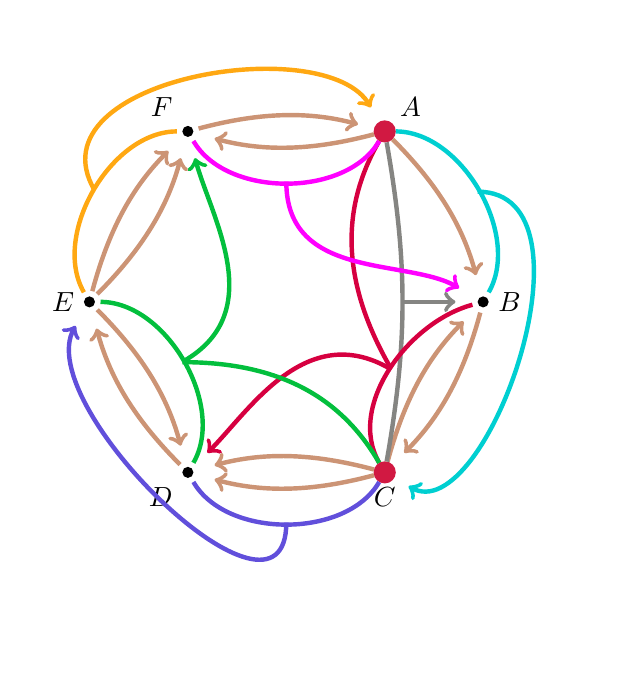
\begin{tikzpicture}
				\def\radius{2.5}
				\coordinate (A) at (60:\radius);
				\coordinate (B) at (0:\radius);
				\coordinate (C) at (300:\radius);
				\coordinate (D) at (240:\radius);
				\coordinate (E) at (180:\radius);
				\coordinate (F) at (120:\radius);
				
				\fill (A) circle (2pt); \node[above right=2pt] at (A) {$A$}; \visible<2->{\fill[alizarin] (A) circle (4pt);}
				\fill (B) circle (2pt); \node[right=2pt] at (B) {$B$};
				\fill (C) circle (2pt); \node[below=2pt] at (C) {$C$}; \visible<2->{\fill[alizarin] (C) circle (4pt);}
				\fill (D) circle (2pt); \node[below left=2pt] at (D) {$D$};
				\fill (E) circle (2pt); \node[left=2pt] at (E) {$E$};
				\fill (F) circle (2pt); \node[above left=2pt] at (F) {$F$};
				
				\visible<-2>{
					\draw[ultra thick, antiquebrass, shorten <= 4pt, shorten >= 10pt, ->] (A) to [out=-45, in=105] (B);
					\draw[ultra thick, antiquebrass, shorten <= 4pt, shorten >= 10pt, ->] (C) to [out=195, in=-15] (D);
					\draw[ultra thick, antiquebrass, shorten <= 4pt, shorten >= 10pt, ->] (D) to [out=135, in=-75] (E);
					\draw[ultra thick, antiquebrass, shorten <= 4pt, shorten >= 10pt, ->] (E) to [out=75, in=-135] (F);
					\draw[ultra thick, antiquebrass, shorten <= 4pt, shorten >= 10pt, ->] (A) to [out=195, in=-15] (F);
					\draw[ultra thick, antiquebrass, shorten <= 4pt, shorten >=10pt, ->] (C) to [out=75, in=-135] (B);
					\draw[ultra thick, antiquebrass, shorten <= 10pt, shorten >= 4pt, <-] (D) to [out=15, in=165] (C);
					\draw[ultra thick, antiquebrass, shorten <= 4pt, shorten >= 10pt, ->] (E) to [out=-45, in=105] (D);
					\draw[ultra thick, antiquebrass, shorten <= 10pt, shorten >= 4pt, <-] (F) to [out=-105, in=45] (E);
				}
				
				\visible<-3>{
					\draw[ultra thick, antiquebrass, shorten <= 4pt, shorten >= 10pt, ->] (B) to [out=-105, in=45] (C);
					\draw[ultra thick, antiquebrass, shorten <= 4pt, shorten >= 10pt, ->] (F) to [out=15, in=165] (A);
				}
				
				\visible<-2>{
					% {AC -> B}
					\draw[ultra thick, battleshipgrey, shorten <= 4pt, shorten >= 4pt] (A) to [out=-80, in=80] node[pos=0.5] (ac)   {} (C);
					\draw[ultra thick, battleshipgrey, shorten <= -4pt, shorten >= 10pt, ->] (ac) to [out = 0, in = 180] (B);
				}
				
				\visible<-3>{
					% {AB -> C}
					\draw[ultra thick, darkturquoise, shorten <= 4pt, shorten >= 4pt] (A) to [out=0, in=60] node[pos=0.5] (ab) {} (B);
					\draw[ultra thick, darkturquoise, shorten <= -4pt, shorten >= 10pt, ->] (ab) to [out = 0, in = -30] (C);
				}
				
				\visible<-2>{
					% {ABC -> D}
					\draw[ultra thick, richcarmine, shorten <= 4pt, shorten >= 4pt] (B) to [out=195, in=120] node[pos=0.5] (bc) {} (C);
					\draw[ultra thick, richcarmine, shorten <= 4pt, shorten >= -4pt] (A) to [out=-120, in=120] (bc);
					\draw[ultra thick, richcarmine, shorten <= -4pt, shorten >= 10pt, ->] (bc) to [out = 150, in = 45] (D);
				}
				
				\visible<-2>{
					% {CD -> E}
					\draw[ultra thick, majorelleblue, shorten <= 4pt, shorten >= 4pt] (C) to [out=240, in=-60] node[pos=0.5] (cd) {} (D);
					\draw[ultra thick, majorelleblue, shorten <= -4pt, shorten >= 10pt, ->] (cd) to [out = -90, in = -120] (E);
				}
				
				\visible<-2>{
					% {CDE -> F}
					\draw[ultra thick, darkpastelgreen, shorten <= 4pt, shorten >= 4pt] (D) to [out=60, in=0] node[pos=0.5] (de) {} (E);
					\draw[ultra thick, darkpastelgreen, shorten <= 4pt, shorten >= -4pt] (C) to [out=120, in=0] (de);
					\draw[ultra thick, darkpastelgreen, shorten <= -4pt, shorten >= 10pt, ->] (de) to [out = 30, in = -75] (F);
				}
				
				\visible<-3>{
					% {EF -> A}
					\draw[ultra thick, darktangerine, shorten <= 4pt, shorten >= 4pt] (E) to [out=120,in=180] node[pos=0.5] (ef) {} (F);
					\draw[ultra thick, darktangerine, shorten <= -4pt, shorten >= 10pt, ->] (ef) to [out = 120, in = 120] (A);
				}
				
				\visible<-2>{
					% {FA -> B}
					\draw[ultra thick, magenta, shorten <= 4pt, shorten >= 4pt] (F) to [out = -60, in = -120] node[pos=0.5] (fa) {} (A);
					\draw[ultra thick, magenta, shorten <= -4pt, shorten >= 10pt, ->] (fa) to [out = -90, in = 150] (B);
				}
			\end{tikzpicture}
		\end{figure}
		
	\end{frame}
	
	\begin{frame}{Out-Degree of $\varnothing\not=\mathsf{X}\subsetneq V$}
		$d^{+}_{\mathcal{H}}(\mathsf{X})$ is the number of hyperarcs $(\mathsf{Y}, v)$ such that $v\not\in\mathsf{X}$ and $\exists u \in \mathsf{Y}\cap\mathsf{X}$.
		\begin{figure}[H]
			\centering
			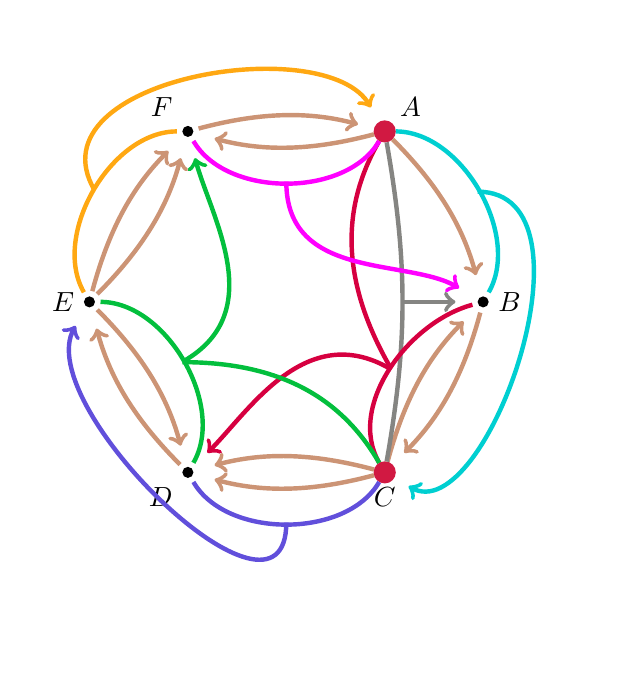
\begin{tikzpicture}
				\def\radius{2.5}
				\coordinate (A) at (60:\radius);
				\coordinate (B) at (0:\radius);
				\coordinate (C) at (300:\radius);
				\coordinate (D) at (240:\radius);
				\coordinate (E) at (180:\radius);
				\coordinate (F) at (120:\radius);
				
				\fill (A) circle (2pt); \node[above right=2pt] at (A) {$A$}; \visible<2->{\fill[alizarin] (A) circle (4pt);}
				\fill (B) circle (2pt); \node[right=2pt] at (B) {$B$};
				\fill (C) circle (2pt); \node[below=2pt] at (C) {$C$}; \visible<2->{\fill[alizarin] (C) circle (4pt);}
				\fill (D) circle (2pt); \node[below left=2pt] at (D) {$D$};
				\fill (E) circle (2pt); \node[left=2pt] at (E) {$E$};
				\fill (F) circle (2pt); \node[above left=2pt] at (F) {$F$};
				
				\visible<-2>{
					\draw[ultra thick, antiquebrass, shorten <= 4pt, shorten >= 10pt, ->] (B) to [out=-105, in=45] (C);
					\draw[ultra thick, antiquebrass, shorten <= 4pt, shorten >= 10pt, ->] (D) to [out=135, in=-75] (E);
					\draw[ultra thick, antiquebrass, shorten <= 4pt, shorten >= 10pt, ->] (E) to [out=75, in=-135] (F);
					\draw[ultra thick, antiquebrass, shorten <= 4pt, shorten >= 10pt, ->] (F) to [out=15, in=165] (A);
					\draw[ultra thick, antiquebrass, shorten <= 4pt, shorten >= 10pt, ->] (E) to [out=-45, in=105] (D);
					\draw[ultra thick, antiquebrass, shorten <= 10pt, shorten >= 4pt, <-] (F) to [out=-105, in=45] (E);
				}
				
				\visible<-3>{
					\draw[ultra thick, antiquebrass, shorten <= 4pt, shorten >= 10pt, ->] (A) to [out=-45, in=105] (B); 
					\draw[ultra thick, antiquebrass, shorten <= 4pt, shorten >= 10pt, ->] (C) to [out=195, in=-15] (D);
					\draw[ultra thick, antiquebrass, shorten <= 4pt, shorten >= 10pt, ->] (A) to [out=195, in=-15] (F);
					\draw[ultra thick, antiquebrass, shorten <= 4pt, shorten >=10pt, ->] (C) to [out=75, in=-135] (B);
					\draw[ultra thick, antiquebrass, shorten <= 10pt, shorten >= 4pt, <-] (D) to [out=15, in=165] (C);
				}
				
				\visible<-3>{
					% {AC -> B}
					\draw[ultra thick, battleshipgrey, shorten <= 4pt, shorten >= 4pt] (A) to [out=-80, in=80] node[pos=0.5]    (ac) {} (C);
					\draw[ultra thick, battleshipgrey, shorten <= -4pt, shorten >= 10pt, ->] (ac) to [out = 0, in = 180] (B);
				}
				
				\visible<-2>{
					% {AB -> C}
					\draw[ultra thick, darkturquoise, shorten <= 4pt, shorten >= 4pt] (A) to [out=0, in=60] node[pos=0.5] (ab) {}   (B);
					\draw[ultra thick, darkturquoise, shorten <= -4pt, shorten >= 10pt, ->] (ab) to [out = 0, in = -30] (C);
				}
				
				\visible<-3>{
					% {ABC -> D}
					\draw[ultra thick, richcarmine, shorten <= 4pt, shorten >= 4pt] (B) to [out=195, in=120] node[pos=0.5] (bc) {} (C);
					\draw[ultra thick, richcarmine, shorten <= 4pt, shorten >= -4pt] (A) to [out=-120, in=120] (bc);
					\draw[ultra thick, richcarmine, shorten <= -4pt, shorten >= 10pt, ->] (bc) to [out = 150, in = 45] (D);
				}
				
				\visible<-3>{
					% {CD -> E}
					\draw[ultra thick, majorelleblue, shorten <= 4pt, shorten >= 4pt] (C) to [out=240, in=-60] node[pos=0.5] (cd)   {} (D);
					\draw[ultra thick, majorelleblue, shorten <= -4pt, shorten >= 10pt, ->] (cd) to [out = -90, in = -120] (E);
				}
				
				\visible<-3>{
					% {CDE -> F}
					\draw[ultra thick, darkpastelgreen, shorten <= 4pt, shorten >= 4pt] (D) to [out=60, in=0] node[pos=0.5] (de) {} (E);
					\draw[ultra thick, darkpastelgreen, shorten <= 4pt, shorten >= -4pt] (C) to [out=120, in=0] (de);
				}
				\draw[ultra thick, darkpastelgreen, shorten <= -4pt, shorten >= 10pt, ->] (de) to [out = 30, in = -75] (F);
				
				\visible<-2>{
					% {EF -> A}
					\draw[ultra thick, darktangerine, shorten <= 4pt, shorten >= 4pt] (E) to [out=120,in=180] node[pos=0.5] (ef) {} (F);
					\draw[ultra thick, darktangerine, shorten <= -4pt, shorten >= 10pt, ->] (ef) to [out = 120, in = 120] (A);
				}
				
				\visible<-3>{
					% {FA -> B}
					\draw[ultra thick, magenta, shorten <= 4pt, shorten >= 4pt] (F) to [out = -60, in = -120] node[pos=0.5] (fa) {} (A);
					\draw[ultra thick, magenta, shorten <= -4pt, shorten >= 10pt, ->] (fa) to [out = -90, in = 150] (B);
				}
				
			\end{tikzpicture}
		\end{figure}
		
	\end{frame}
	
	\begin{frame}{Hyperarc-connectivity}
		\begin{itemize}[<+->]
			\item $\vec{\mathcal{H}}$ is \textit{$k$-hyperarc-connected}, if, $\forall\varnothing\not=X\subsetneq V$, $d^{+}_{\vec{\mathcal{H}}}(X) \geq k$.
			\item The hyperarc-connectivity of a hypergraph, denoted $\lambda(\vec{\mathcal{H}})$, is the maximum value of $k$ such that $\vec{\mathcal{H}}$ is \textit{$k$-hyperarc-connected}.
		\end{itemize}
	\end{frame}
	
	\section{Principal results}
	\begin{frame}{Main result}
		We use a result of Frank : $\mathcal{H}$ is $(k, k)$-partition-connected if and only if it admits a $k$-hyperarc-connected orientation.

		\begin{tcolorbox}[colback=richcarmine!5!white,colframe=richcarmine!75!black,title=Main result (Theorem 7)]
			Let $\mathcal{H} = (V, E)$ be a $(k+1, k+1)$-partition-connected hypergraph and $\vec{\mathcal{H}}$ is a k-hyperarc connected orientation of $\mathcal{H}$. Then there exists a sequence of hypergraphs $(\vec{\mathcal{H}_{i}})_{i\in0\dots\ell}$ such that $\vec{\mathcal{H}}_{i+1}$ is obtained from $\vec{\mathcal{H}}_{i}$ by reorienting exactly one hyperarc and $\lambda(\vec{\mathcal{H}}_{i+1}) \geq \lambda(\vec{\mathcal{H}}_{i})$ and $\lambda(\vec{\mathcal{H}}_{\ell}) = k + 1$. Such a sequence of orientations can be obtained with $\ell \leq |V|^{3}$ and found in polynomial time (in the size of $\mathcal{H}$).
		\end{tcolorbox}
	\end{frame}
	
	\begin{frame}{"High-Level"-running of the algorithm}
		Our algorithm will provide a 3-hyperarc-connected orientation of $\mathcal{H}$, starting from a 2-hyperarc-connected.
		
		\begin{columns}
			\begin{column}{0.5\textwidth}
				\begin{figure}[H]
					\centering
					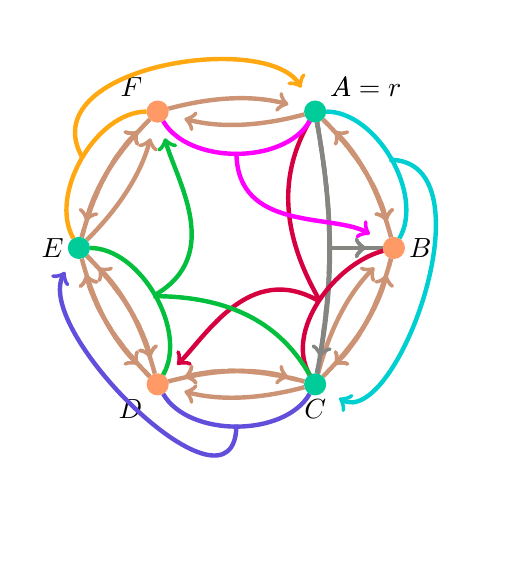
\begin{tikzpicture}
						\def\radius{2}
						\coordinate (A) at (60:\radius);
						\coordinate (B) at (0:\radius);
						\coordinate (C) at (300:\radius);
						\coordinate (D) at (240:\radius);
						\coordinate (E) at (180:\radius);
						\coordinate (F) at (120:\radius);
						
						\fill (A) circle (2pt);
							\visible<1>{\node[above right=2pt] at (A) {$A$};}
							\visible<2->{\node[above right=2pt] at (A) {$A = r$};}
							\visible<18-23>{\fill[caribbeangreen] (A) circle (4pt);}
						
						\fill (B) circle (2pt);
							\node[right=2pt] at (B) {$B$};
							\visible<6>{\fill[atomictangerine] (B) circle (4pt);}

						\fill (C) circle (2pt);
							\node[below=2pt] at (C) {$C$};
							\visible<6>{\fill[caribbeangreen] (C) circle (4pt);}

						\fill (D) circle (2pt);
							\node[below left=2pt] at (D) {$D$};
							\visible<12>{\fill[atomictangerine] (D) circle (4pt);}
						
						\fill (E) circle (2pt);
							\node[left=2pt] at (E) {$E$};
							\visible<12>{\fill[caribbeangreen] (E) circle (4pt);}

						\fill (F) circle (2pt);
							\node[above left=2pt] at (F) {$F$};
							\visible<18-23>{\fill[atomictangerine] (F) circle (4pt);}
						
						\draw[ultra thick, antiquebrass, shorten <= 4pt, shorten >= 10pt, ->] (C) to [out=195, in=-15] (D);
						\draw[ultra thick, antiquebrass, shorten <= 4pt, shorten >= 10pt, ->] (F) to [out=15, in=165] (A);
						\draw[ultra thick, antiquebrass, shorten <= 4pt, shorten >= 10pt, ->] (A) to [out=195, in=-15] (F);
						\draw[ultra thick, antiquebrass, shorten <= 4pt, shorten >=10pt, ->] (C) to [out=75, in=-135] (B);	
						\draw[ultra thick, antiquebrass, shorten <= 10pt, shorten >= 4pt, <-] (F) to [out=-105, in=45] (E);

						\visible<-11>{
							\draw[ultra thick, antiquebrass, shorten <= 4pt, shorten >= 10pt, ->] (E) to [out=-45, in=105] (D);
						}
						\visible<12>{
							\draw[dashdotted, ultra thick, antiquebrass, shorten <= 4pt, shorten >= 10pt, ->] (E) to [out=-45, in=105] (D);
						}
						\visible<13->{
							\draw[ultra thick, antiquebrass, shorten <= 10pt, shorten >= 4pt, <-] (E) to [out=-45, in=105] (D);
						}

						% {AC -> B}
						\visible<-5>{
							\draw[ultra thick, battleshipgrey, shorten <= 4pt, shorten >= 4pt] (A) to [out=-80, in=80] node[pos=0.5] (ac) {} (C);
							\draw[ultra thick, battleshipgrey, shorten <= -4pt, shorten >= 10pt, ->] (ac) to [out = 0, in = 180] (B);
						}
						\visible<6>{
							\draw[dashdotted, ultra thick, battleshipgrey, shorten <= 4pt, shorten >= 4pt] (A) to [out=-80, in=80] node[pos=0.5] (ac) {} (C);
							\draw[dashdotted, ultra thick, battleshipgrey, shorten <= -4pt, shorten >= 10pt, ->] (ac) to [out = 0, in = 180] (B);
						}
						\visible<7->{
							\draw[ultra thick, battleshipgrey, shorten <= 4pt, shorten >= 10pt, ->] (A) to [out=-80, in=80] node[pos=0.5] (ac) {} (C);
							\draw[ultra thick, battleshipgrey, shorten <= -4pt, shorten >= 4pt] (ac) to [out = 0, in = 180] (B);
						}

						% TODO : Highlight @ step 18, reorient step by step (19 -> 23)
						\visible<-17>{
							\draw[ultra thick, antiquebrass, shorten <= 4pt, shorten >= 10pt, ->] (A) to [out=-45, in=105] (B);
							\draw[ultra thick, antiquebrass, shorten <= 4pt, shorten >= 10pt, ->] (B) to [out=-105, in=45] (C);
							\draw[ultra thick, antiquebrass, shorten <= 10pt, shorten >= 4pt, <-] (D) to [out=15, in=165] (C);
							\draw[ultra thick, antiquebrass, shorten <= 4pt, shorten >= 10pt, ->] (D) to [out=135, in=-75] (E);
							\draw[ultra thick, antiquebrass, shorten <= 4pt, shorten >= 10pt, ->] (E) to [out=75, in=-135] (F);
						}
						\visible<18-22>{\draw[dashdotted, ultra thick, antiquebrass, shorten <= 4pt, shorten >= 10pt, ->] (A) to [out=-45, in=105] (B);}
						\visible<18-21>{\draw[dashdotted, ultra thick, antiquebrass, shorten <= 4pt, shorten >= 10pt, ->] (B) to [out=-105, in=45] (C);}
						\visible<18-20>{\draw[dashdotted, ultra thick, antiquebrass, shorten <= 10pt, shorten >= 4pt, <-] (D) to [out=15, in=165] (C);}
						\visible<18-19>{\draw[dashdotted, ultra thick, antiquebrass, shorten <= 4pt, shorten >= 10pt, ->] (D) to [out=135, in=-75] (E);}
						\visible<18-18>{\draw[dashdotted, ultra thick, antiquebrass, shorten <= 4pt, shorten >= 10pt, ->] (E) to [out=75, in=-135] (F);}
				
						\visible<23->{\draw[ultra thick, antiquebrass, shorten <= 10pt, shorten >= 4pt, <-] (A) to [out=-45, in=105] (B);}
						\visible<22->{\draw[ultra thick, antiquebrass, shorten <= 10pt, shorten >= 4pt, <-] (B) to [out=-105, in=45] (C);}
						\visible<21->{\draw[ultra thick, antiquebrass, shorten <= 4pt, shorten >= 10pt, ->] (D) to [out=15, in=165] (C);}
						\visible<20->{\draw[ultra thick, antiquebrass, shorten <= 10pt, shorten >= 4pt, <-] (D) to [out=135, in=-75] (E);}
						\visible<19->{\draw[ultra thick, antiquebrass, shorten <= 10pt, shorten >= 4pt, <-] (E) to [out=75, in=-135] (F);}

						% {AB -> C}
						\draw[ultra thick, darkturquoise, shorten <= 4pt, shorten >= 4pt] (A) to [out=0, in=60] node[pos=0.5] (ab) {} (B);
						\draw[ultra thick, darkturquoise, shorten <= -4pt, shorten >= 10pt, ->] (ab) to [out = 0, in = -30] (C);
						
						% {ABC -> D}
						\draw[ultra thick, richcarmine, shorten <= 4pt, shorten >= 4pt] (B) to [out=195, in=120] node[pos=0.5] (bc) {} (C);
						\draw[ultra thick, richcarmine, shorten <= 4pt, shorten >= -4pt] (A) to [out=-120, in=120] (bc);
						\draw[ultra thick, richcarmine, shorten <= -4pt, shorten >= 10pt, ->] (bc) to [out = 150, in = 45] (D);
						
						% {CD -> E}
						\draw[ultra thick, majorelleblue, shorten <= 4pt, shorten >= 4pt] (C) to [out=240, in=-60] node[pos=0.5] (cd) {} (D);
						\draw[ultra thick, majorelleblue, shorten <= -4pt, shorten >= 10pt, ->] (cd) to [out = -90, in = -120] (E);
						
						% {CDE -> F}
						\draw[ultra thick, darkpastelgreen, shorten <= 4pt, shorten >= 4pt] (D) to [out=60, in=0] node[pos=0.5] (de) {} (E);
						\draw[ultra thick, darkpastelgreen, shorten <= 4pt, shorten >= -4pt] (C) to [out=120, in=0] (de);
						
						\draw[ultra thick, darkpastelgreen, shorten <= -4pt, shorten >= 10pt, ->] (de) to [out = 30, in = -75] (F);
						
						% {EF -> A}
						\draw[ultra thick, darktangerine, shorten <= 4pt, shorten >= 4pt] (E) to [out=120,in=180] node[pos=0.5] (ef) {} (F);
						\draw[ultra thick, darktangerine, shorten <= -4pt, shorten >= 10pt, ->] (ef) to [out = 120, in = 120] (A);
						
						% {FA -> B}
						\draw[ultra thick, magenta, shorten <= 4pt, shorten >= 4pt] (F) to [out = -60, in = -120] node[pos=0.5] (fa) {} (A);
						\draw[ultra thick, magenta, shorten <= -4pt, shorten >= 10pt, ->] (fa) to [out = -90, in = 150] (B);
						
					\end{tikzpicture}
				\end{figure}
			\end{column}
			\hfill
			\begin{column}{0.5\textwidth}
				\begin{enumerate}
					\item <alert@2> Take $r$ in $V(\mathcal{H})$.
					\item <alert@3,9,15,25> Compute sets of vertices.
					\item <alert@4,10,16,26> Stopping Criteria
					\item <alert@5,11,17> Select a set $R$ (cf. 2.)
					\item <alert@6,12,18> Find an admissible $({\color{caribbeangreen}s}, {\color{atomictangerine}t})$-hyperpath in $R$ to reorient
					\item <alert@7,13,19-23> Reorient the corresponding hyperpath.
					\item <alert@8,14,24> \texttt{Goto} (2.)
				\end{enumerate}
			\end{column}
		\end{columns}	
	\end{frame}

	\begin{frame}{Finding \textit{admissible} $(s, t)$-hyperpaths in $R$}

		\begin{tcolorbox}[colback=darkseagreen!5!white,colframe=darkseagreen!75!black,title=Admissible hyperpaths]
			\begin{itemize}[<+->]
				\item Three criterion for $P$ to be an admissible $(s, t)$-hyperpath in $R$:
				\begin{itemize}
					\item[1.] \textit{Stopping Criteria}-related argument
					\item[2.] $s$ is a {\color{alizarin}safe source} in $S\subseteq{R}$, $t$ is a {\color{alizarin}safe sink} in $T\subseteq{R}$.
					\item[3.] Reorient each hyperarc, \textbf{one by one}, does not decrease the hyperarc-connectivity.
				\end{itemize}
			\end{itemize}
		\end{tcolorbox}

		\begin{flushright}
			\textit{A brief detour...}
		\end{flushright}
	\end{frame}

	\section{Setting up the framework}
	\begin{frame}{Tight and Minimal-tight sets}
		\begin{columns}
			\begin{column}{0.45\textwidth}
				\begin{figure}[H]
					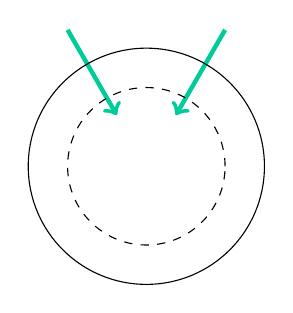
\begin{tikzpicture}
						\def\radius{0.75}
						\def\smol{1}
						\def\mid{1.5}
						\def\Radius{2}

						\coordinate (u) at (120:\radius);
						\coordinate (U) at (120:\Radius);

						\coordinate (w) at (60:\radius);
						\coordinate (W) at (60:\Radius);
					
						\draw[ultra thick, ->, caribbeangreen] (U) to [out=-60, in=120] (u);
						\draw[ultra thick, ->, caribbeangreen] (W) to [out=-120, in=60] (w);
						
						\visible<1,3>{\draw[thin] (0,0) circle (\mid);}
						\visible<2,3>{\draw[thin, dashed] (0,0) circle (\smol);}
									
					\end{tikzpicture}

					\caption*{\only<2>{Minimal }In-\only<1->{Tight} sets}
				\end{figure}
			\end{column}
			\hfill\vrule\hfill
			\begin{column}{0.45\textwidth}
				\begin{figure}[H]
					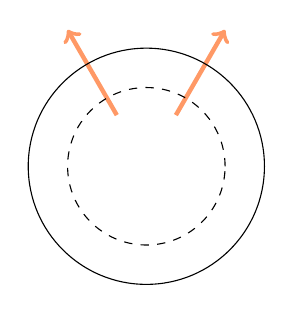
\begin{tikzpicture}
						\def\radius{0.75}
						\def\smol{1}
						\def\mid{1.5}
						\def\Radius{2}

						\coordinate (u) at (120:\radius);
						\coordinate (U) at (120:\Radius);
						\coordinate (w) at (60:\radius);
						\coordinate (W) at (60:\Radius);
					
						\draw[ultra thick, <-, atomictangerine] (U) to [out=-60, in=120] (u);
						\draw[ultra thick, <-, atomictangerine] (W) to [out=-120, in=60] (w);
						
						\visible<1,3>{\draw[thin] (0,0) circle (\mid);}
						\visible<2,3>{\draw[thin, dashed] (0,0) circle (\smol);}				
					\end{tikzpicture}
					\caption*{\only<2>{Minimal }Out-\only<1->{Tight} sets}
				\end{figure}
			\end{column}
		\end{columns}

		\begin{itemize}[<+->]
			\item<1,3> ${\color{caribbeangreen}\mathcal{T}_{-}} = \{X \subseteq V - r, d^{-}(X) = k\} \cup \{V\}$
			\item<1,3> ${\color{atomictangerine}\mathcal{T}_{+}} = \{X \subseteq V - r, d^{+}(X) = k\} \cup \{V\}$
			\item<2,3> ${\color{caribbeangreen}\mathcal{M}_{-}}$ : Inclusion-wise minimal members of ${\color{caribbeangreen}\mathcal{T}_{-}}$
			\item<2,3> ${\color{atomictangerine}\mathcal{M}_{+}}$ : Inclusion-wise minimal members of ${\color{atomictangerine}\mathcal{T}_{+}}$
		\end{itemize}

	\end{frame}

	\begin{frame}{Crossing sets and structural results}
		\begin{tcolorbox}[colback=bondiblue!5!white,colframe=bondiblue!75!black,title=Claim 1(b)]	
		Let $X, Y$ two crossing sets in $V$.\\
		If $X, Y\in{\color{atomictangerine}\mathcal{T}_{+}}$, then both $X\cup{Y}\in{\color{atomictangerine}\mathcal{T}_{+}}$ and $X\cap{Y}\in{\color{atomictangerine}\mathcal{T}_{+}}$.
		\end{tcolorbox}

		\begin{block}{Proof of Claim 1(b)}
			\begin{itemize}[<+->]
				\item Since $X, Y$ are crossing, $X\cap{Y}\not=\varnothing$, $X\cup{Y}\not=V$.
				\item $k + k = d^{+}(X) + d^{+}(Y)$
				\item By submodularity, $d^{+}(X) + d^{+}(Y) \geq d^{+}(X\cup{Y}) + d^{+}(X\cap{Y})$
				\item As $\lambda(\vec{\mathcal{H}}) = k$, we have $d^{+}(X\cup{Y}) \geq k$ and $d^{+}(X\cap{Y}) \geq k$
				\item Grouping these equations, we obtain : $k + k = d^{+}(X) + d^{+}(Y) \geq d^{+}(X\cup{Y}) + d^{+}(X\cap{Y}) \geq k + k$.
				\item This implies $d^{+}(X\cup Y) = k = d^{+}(X\cap Y)$, i.e. $X\cap Y, X\cup Y \in {\color{atomictangerine}\mathcal{T}_{+}}$
			\end{itemize}
		\end{block}
	\end{frame}

	\mode<handout>{
		\begin{frame}{Safe Sources and Safe Sinks}
			Definitions are symmetric (but proofs are not).
			\only<1-2>{\begin{itemize}
				\item For $S \in \mathcal{M}_{-}$, $s$ is a safe source in $S$ if :\begin{itemize}
					\item[a]<1,2>{For every $s\in{X}\in\mathcal{T}_{+}$, we have $\color{red} S\subsetneq X$.}
					\item[b]<2>{For every $s\in{X}\in\mathcal{D}_{+}$ such that $S\setminus{X}\not=\varnothing$, there exists $Y\in\mathcal{T}_{+}$ such that $s\not\in{Y}\subsetneq{X}$.}
				\end{itemize}
			\end{itemize}
			\begin{columns}
				\begin{column}{0.35\textwidth}
					\only<1,2>{
						\begin{figure}[H]
							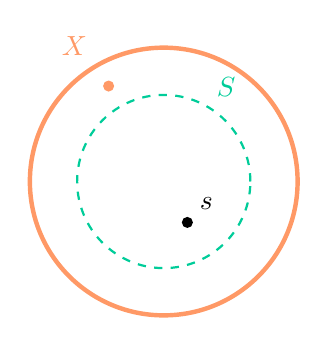
\begin{tikzpicture}
								\def\smolrad{0.6}
								\def\midrad{1.1}
								\def\intrad{1.4}
								\def\bigrad{1.7}

								\coordinate (s) at (-60:\smolrad);
								\fill (s) circle (2pt);
								\node[above right=1pt] at (s) {$s$};

								\coordinate (S) at (60:\midrad);
								\node[above right] at (S) {$\color{caribbeangreen}S$};

								\coordinate (X) at (120:\bigrad);
								\node[above left] at (X) {$\color{atomictangerine}{X}$};

								\coordinate (x) at (120:\intrad);
								\fill[atomictangerine] (x) circle (2pt);

								\draw[thick, caribbeangreen, dashed] (0,0) circle (\midrad);
								\draw[ultra thick, atomictangerine] (0,0) circle (\bigrad);
							\end{tikzpicture}
							\caption*{Condition (a)}
						\end{figure}
					}
				\end{column}
				\hfill\vrule\hfill
				\begin{column}{0.60\textwidth}
					\only<2>{
						\begin{figure}[H]
							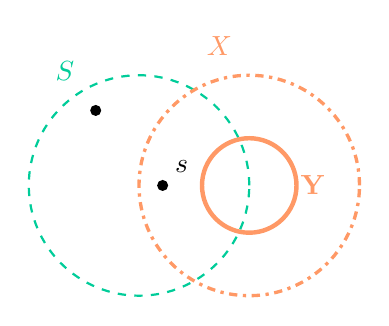
\begin{tikzpicture}
								\def\ssmolrad{0.3}
								\def\smolrad{0.6}
								\def\midrad{1.1}
								\def\intrad{1.4}
								\def\bigrad{1.7}

								\coordinate (s) at (0:\ssmolrad);
								\fill (s) circle (2pt);
								\node[above right=1pt] at (s) {$s$};

								\coordinate (S) at (120:\intrad);
								\node[above left] at (S) {$\color{caribbeangreen}S$};

								\fill(120:\midrad) circle (2pt);

								\node at (60:{1.2*\bigrad}) {$\color{atomictangerine}X$};
								\node at (0:{1.3*\bigrad}) {$\color{atomictangerine}\mathbf{Y}$};
								
								\draw[thick, caribbeangreen, dashed] (0,0) circle (\intrad);

								\coordinate (cE) at (0:\intrad);
								\draw[very thick, atomictangerine, dashdotted] (cE) circle (\intrad);
								\draw[ultra thick, atomictangerine] (cE) circle (\smolrad);
							\end{tikzpicture}
							\caption*{Condition (b)}
						\end{figure}
					}
				\end{column}
			\end{columns}
			}
			\only<3>{\begin{itemize}
				\item For $T \in \mathcal{M}_{+}$, $t$ is a safe sink in $T$ if :\begin{itemize}
					\item[c]{For every $t\in{X}\in\mathcal{T}_{-}$, we have $\color{red}T\subsetneq X$.}
					\item[d]{For every $t\in{X}\in\mathcal{D}_{-}$ such that $T\setminus{X}\not=\varnothing$, there exists $Y\in\mathcal{T}_{-}$ such that $t\not\in{Y}\subsetneq{X}$.}
				\end{itemize}
			\end{itemize}
			\begin{columns}
				\begin{column}{0.35\textwidth}
					\begin{figure}[H]
						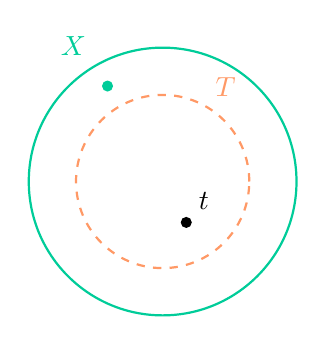
\begin{tikzpicture}
							\def\smolrad{0.6}
							\def\midrad{1.1}
							\def\intrad{1.4}
							\def\bigrad{1.7}

							\coordinate (t) at (-60:\smolrad);
							\fill (t) circle (2pt);
							\node[above right=1pt] at (t) {$t$};

							\coordinate (T) at (60:\midrad);
							\node[above right] at (T) {$\color{atomictangerine}T$};

							\coordinate (X) at (120:\bigrad);
							\node[above left] at (X) {$\color{caribbeangreen}{X}$};

							\coordinate (x) at (120:\intrad);
							\fill[caribbeangreen] (x) circle (2pt);

							\draw[thick, atomictangerine, dashed] (0,0) circle (\midrad);
							\draw[thick, caribbeangreen] (0,0) circle (\bigrad);
						\end{tikzpicture}
						\caption*{Condition (c)}
					\end{figure}
				\end{column}
				\hfill\vrule\hfill
				\begin{column}{0.60\textwidth}
					\begin{figure}[H]
						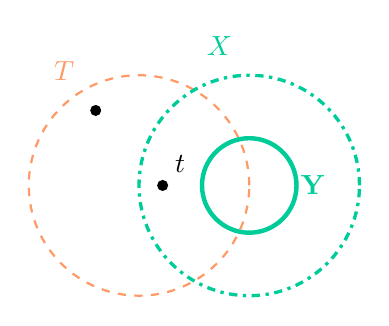
\begin{tikzpicture}
							\def\ssmolrad{0.3}
							\def\smolrad{0.6}
							\def\midrad{1.1}
							\def\intrad{1.4}
							\def\bigrad{1.7}

							\coordinate (t) at (0:\ssmolrad);
							\fill (t) circle (2pt);
							\node[above right=1pt] at (t) {$t$};

							\coordinate (T) at (120:\intrad);
							\node[above left] at (T) {$\color{atomictangerine}T$};

							\fill(120:\midrad) circle (2pt);

							\node at (60:{1.2*\bigrad}) {$\color{caribbeangreen}X$};
							\node at (0:{1.3*\bigrad}) {$\color{caribbeangreen}\mathbf{Y}$};
							
							\draw[thick, atomictangerine, dashed] (0,0) circle (\intrad);

							\coordinate (cE) at (0:\intrad);
							\draw[very thick, caribbeangreen, dashdotted] (cE) circle (\intrad);
							\draw[ultra thick, caribbeangreen] (cE) circle (\smolrad);
						\end{tikzpicture}
						\caption*{Condition (d)}
					\end{figure}
				\end{column}
			\end{columns}
			}
			Finding a safe sink $t$ in $T\in\mathcal{M}_{+}$ can be done by checking each vertex if they correspond to the definition.
		\end{frame}
	}

	\begin{frame}{Finding \textit{admissible} $(s, t)$-hyperpaths in $R$}

		\begin{tcolorbox}[colback=darkseagreen!5!white,colframe=darkseagreen!75!black,title=Admissible hyperpaths]
			Three criterion for $P$ to be an admissible $(s, t)$-hyperpath in $R$:	
			\begin{itemize}
				\item[1.] Stopping criteria for the main algorithm :
				\item[2.] $s$ is a safe source in $S\subseteq{R}$, $t$ is a safe sink in $T\subseteq{R}$.
				\item[3.] Reorienting each hyperarc, \textbf{one by one}, does not decrease the hyperarc-connectivity
			\end{itemize}
		\end{tcolorbox}
		
		\begin{itemize}
			\item Stopping criteria : ${\color{caribbeangreen}\mathcal{M}_{-}} = \{V\}$ and ${\color{atomictangerine}\mathcal{M}_{+}} = \{V\}$.
			\item ${\color{caribbeangreen}\mathcal{T}_{-}} = \{X \subseteq V - r, d^{-}(X) = k\} \cup \{V\}$
			\item ${\color{caribbeangreen}\mathcal{M}_{-}}$ : Inclusion-wise minimal members of ${\color{caribbeangreen}\mathcal{T}_{-}}$
			\item Finally, if $\lambda(\vec{\mathcal{H}}) \geq k$ and ${\color{caribbeangreen}\mathcal{T}_{-}} = {\color{atomictangerine}\mathcal{T}_{+}} = \{V\}$, $\vec{\mathcal{H}}$ is $(k+1)$-hyperarc-connected.
		\end{itemize}
	\end{frame}

	\begin{frame}{Existence of a safe source (\textit{a safe sink})}
		\begin{tcolorbox}[colback=lightsalmon!5!white,colframe=lightsalmon!75!black,title=Lemma 10]
			$\forall{S}\in{\color{caribbeangreen}\mathcal{M}_{-}}, \text{ there is a safe source }s\in{S}.$
		\end{tcolorbox}

		\begin{tcolorbox}[colback=lightsalmon!5!white,colframe=lightsalmon!75!black,title=Lemma 11]
			$\forall{T}\in{\color{atomictangerine}\mathcal{M}_{+}}, \text{ there is a safe sink }t\in{T}.$
		\end{tcolorbox}
	\end{frame}

	\section{Towards $(k+1)$-hyperarc connectivity}
	\begin{frame}{Towards hyperarc connectivity augmentation}
		$\mathcal{R}$ : $R\subseteq V - r$ inclusion-wise minimal such that either :
		\begin{itemize}
			\item $R\in{\color{caribbeangreen}\mathcal{T}_{-}}$, and contains a member of ${\color{atomictangerine}\mathcal{T}_{+}}$
			\item or $R\in{\color{atomictangerine}\mathcal{T}_{+}}$, and contains a member of ${\color{caribbeangreen}\mathcal{T}_{-}}$.
		\end{itemize}

		\begin{tcolorbox}[colback=lightsalmon!5!white,colframe=lightsalmon!75!black,title=Lemma 13]
			Let $R\in\mathcal{R}, S\in{\color{caribbeangreen}\mathcal{M}_{-}}, T\in{\color{atomictangerine}\mathcal{M}_{+}}$ such that $S,T\subseteq{R}$. Let $s$ be a safe source in $S$, $t$ a safe sink in $T$.
			\begin{itemize}
				\item[a.] $\forall{X}\subseteq V-r$ such that $s\in X$, $t\not\in X$, we have $d^{+}(X) \geq k + 1$.
				\item[b.] $\forall{X}\subseteq V-r$ such that $s\not\in X$, $t\in X$, we have $d^{-}(X) \geq k + 1$.
			\end{itemize}
		\end{tcolorbox}

		\begin{columns}
			\begin{column}{0.45\textwidth}
				\begin{figure}[H]
					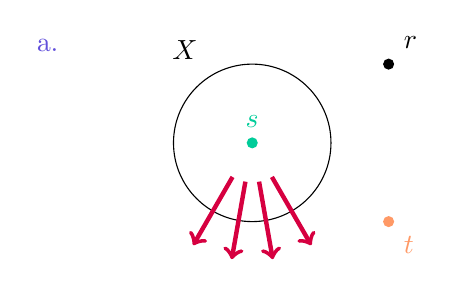
\begin{tikzpicture}
						\def\sadius{0.5}
						\def\radius{1}
						\def\madius{1.5}
						\def\Radius{2}

						\coordinate (a) at (150:{3*\radius});
						\node[below = 2pt] at (a) {{\color{majorelleblue}a.}};

						\coordinate (s) at (0, 0);
						\fill[caribbeangreen] (s) circle (2pt);
						\node[above = 2pt] at (s) {${\color{caribbeangreen}s}$};
						
						\coordinate (X) at (120:\radius);
						\node[above left = 2pt] at (X) {$X$};

						\coordinate (r) at (30:\Radius);
						\fill (r) circle (2pt);
						\node[above right = 2pt] at (r) {$r$};

						\coordinate (t) at (-30:\Radius);
						\fill[atomictangerine] (t) circle (2pt);
						\node[below right = 2pt] at (t) {$\color{atomictangerine}t$};

						\draw[thin] (0,0) circle (\radius);

						\coordinate (o1) at (-60:\sadius);
						\coordinate (o2) at (-80:\sadius);
						\coordinate (o3) at (-100:\sadius);
						\coordinate (o4) at (-120:\sadius);

						\coordinate (O1) at (-60:\madius);
						\coordinate (O2) at (-80:\madius);
						\coordinate (O3) at (-100:\madius);
						\coordinate (O4) at (-120:\madius);

						\draw[ultra thick, ->, richcarmine] (o1) -- (O1);
						\draw[ultra thick, ->, richcarmine] (o2) -- (O2);
						\draw[ultra thick, ->, richcarmine] (o3) -- (O3);
						\draw[ultra thick, ->, richcarmine] (o4) -- (O4);	
					\end{tikzpicture}
				\end{figure}
			\end{column}
			\hfill\vrule\hfill
			\begin{column}{0.45\textwidth}
				\begin{figure}[H]
					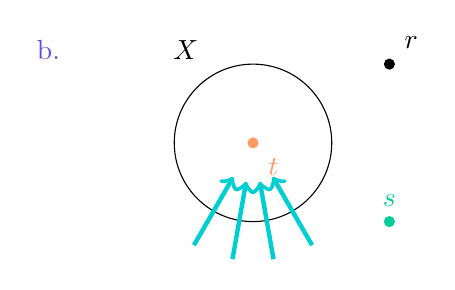
\begin{tikzpicture}
						\def\sadius{0.5}
						\def\radius{1}
						\def\madius{1.5}
						\def\Radius{2}

						\coordinate (b) at (150:{3*\radius});
						\node[below = 2pt] at (b) {{\color{majorelleblue}b.}};

						\coordinate (s) at (-30:\Radius);
						\fill[caribbeangreen] (s) circle (2pt);
						\node[above = 2pt] at (s) {${\color{caribbeangreen}s}$};
						
						\coordinate (X) at (120:\radius);
						\node[above left = 2pt] at (X) {$X$};

						\coordinate (r) at (30:\Radius);
						\fill (r) circle (2pt);
						\node[above right = 2pt] at (r) {$r$};

						\coordinate (t) at (0, 0);
						\fill[atomictangerine] (t) circle (2pt);
						\node[below right = 2pt] at (t) {$\color{atomictangerine}t$};

						\draw[thin] (0,0) circle (\radius);

						\coordinate (o1) at (-60:\sadius);
						\coordinate (o2) at (-80:\sadius);
						\coordinate (o3) at (-100:\sadius);
						\coordinate (o4) at (-120:\sadius);

						\coordinate (O1) at (-60:\madius);
						\coordinate (O2) at (-80:\madius);
						\coordinate (O3) at (-100:\madius);
						\coordinate (O4) at (-120:\madius);

						\draw[ultra thick, <-, darkturquoise] (o1) -- (O1);
						\draw[ultra thick, <-, darkturquoise] (o2) -- (O2);
						\draw[ultra thick, <-, darkturquoise] (o3) -- (O3);
						\draw[ultra thick, <-, darkturquoise] (o4) -- (O4);	
					\end{tikzpicture}
				\end{figure}
			\end{column}
		\end{columns}
	\end{frame}

	\begin{frame}{Towards hyperarc connectivity augmentation}
		\begin{tcolorbox}[colback=lightsalmon!5!white,colframe=lightsalmon!75!black,title=Lemma 13]
			Let $R\in\mathcal{R}, S\in{\color{caribbeangreen}\mathcal{M}_{-}}, T\in{\color{atomictangerine}\mathcal{M}_{+}}$ such that $S,T\subseteq{R}$. Let $s$ be a safe source in $S$, $t$ a safe sink in $T$.
			\begin{itemize}
				\item[a.] $\forall{X}\subseteq V-r$ such that $s\in X$, $t\not\in X$, we have $d^{+}(X) \geq k + 1$.
				\item[b.] $\forall{X}\subseteq V-r$ such that $s\not\in X$, $t\in X$, we have $d^{-}(X) \geq k + 1$.
			\end{itemize}
		\end{tcolorbox}
		
		\begin{block}{Proof of Lemma 13}
			By contradiction, either :
			\begin{itemize}
				\item[\textbf<2>{\color<2>{alizarin}a.}] $\exists X\subseteq V - r, s\in X, t\not\in X, d^{+}(X) = k$, i.e. $s\in X, t\not\in X, X\in{\color{atomictangerine}\mathcal{T}_{+}}$.{\begin{itemize}
					\item[\textbf<2>{\color<2>{alizarin}a1.}] $R\in\mathcal{R}\cap{\color{caribbeangreen}\mathcal{T}_{-}}$
					\item[\textbf<2>{\color<2>{alizarin}a2.}] $R\in\mathcal{R}\cap{\color{atomictangerine}\mathcal{T}_{+}}$ 
				\end{itemize}}
				\item[b.] $\exists{X}\subseteq{V-r}, s\not\in X, t\in X, d^{-}(X) = k$, i.e. $s\not\in X, t\in X, X\in{\color{caribbeangreen}\mathcal{T}_{-}}$.{\begin{itemize}
					\item[b1.] $R\in\mathcal{R}\cap{\color{caribbeangreen}\mathcal{T}_{-}}$
					\item[b2.] $R\in\mathcal{R}\cap{\color{atomictangerine}\mathcal{T}_{+}}$ 
				\end{itemize}}
			\end{itemize}
		\end{block}
	\end{frame}

	\begin{frame}{Proof of Lemma 13}
		${\color{majorelleblue}a} : \exists X\subseteq V-r, s\in{X}, t\not\in{X}, X\in{\color{atomictangerine}\mathcal{T}_{+}}$\\
		
		\begin{itemize}
			\item[.] Since $s\in{S}$ is a \textbf{safe source} and $s\in{X}\in{\color{atomictangerine}\mathcal{T}_{+}}$, we have $S\subsetneq X$
			\item[.] We also have $t\in R\setminus{X}$ by [{\color{majorelleblue}a.}], so $X\setminus{R} \not= \varnothing$.
		\end{itemize}

		\begin{figure}[H]
			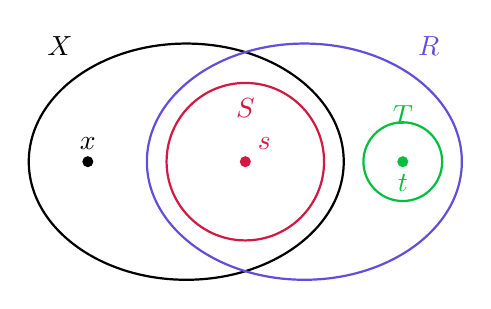
\begin{tikzpicture}
				\def\smolrad{0.5}
				\def\radius{1}
				\def\Radius{1.5}
				\def\bigrad{2}

				\coordinate (s) at (0, 0);
				\fill[alizarin] (s) circle (2pt);
				\node[above right = 1pt] at (s) {${\color{alizarin}s}$};
				\draw[alizarin, thick] (s) circle (\radius);

				\coordinate (cx) at (-0.75, 0);
				\draw[thick] (cx) ellipse (20mm and 15mm);

				\coordinate (x) at (-2, 0);
				\fill (x) circle (2pt);
				\node[above = 1pt] at (x) {$x$};

				\coordinate(X) at (-2, 1.15);
				\node[above left = 2pt] at (X) {$X$};

				\coordinate (cr) at (0.75, 0);
				\draw[majorelleblue, thick] (cr) ellipse (20mm and 15mm);

				\coordinate(S) at (0, 1);
				\node[below = 2pt] at (S) {${\color{alizarin}S}$};

				\coordinate(R) at (2, 1.15);
				\node[above right = 2pt] at (R) {${\color{majorelleblue}R}$};

				\coordinate (t) at (2, 0);
				\fill[darkpastelgreen] (t) circle (2pt);
				\node[below = 1pt] at (t) {${\color{darkpastelgreen}t}$};

				\visible<2>{
					\draw[darkpastelgreen, thick] (t) circle (\smolrad);
					\node[above = 1em] at (t) {${\color{darkpastelgreen}T}$};
				}
			\end{tikzpicture}
			\caption*{Proper representation of ${\color{majorelleblue}a}$}
		\end{figure}

		\only<2>{
			${\color{majorelleblue}a1.} : R\in\mathcal{R}\cap{\color{caribbeangreen}\mathcal{T}_{-}}, \exists X\subseteq V-r, s\in{X}, t\not\in{X}, X\in{\color{atomictangerine}\mathcal{T}_{+}}$.
			\begin{itemize}
				\item[.] As $t\in R\setminus X \not=\varnothing$, and using \textsf{Claim 1}, we have $R\setminus X \in {\color{caribbeangreen}\mathcal{T}_{-}}$.
				\item[.] $T\cap{X} \not= \varnothing$ would contradict the minimality of $T$, so $T$ and $X$ are disjoint.
				\item[.] As $R\setminus{X} \in {\color{caribbeangreen}\mathcal{T}_{-}}$, $T\in{\color{atomictangerine}\mathcal{T}_{+}}$, and $T\subseteq R\setminus{X}$, this contradicts $R$ minimal.
			\end{itemize}
		}

		\only<3>{
			${\color{majorelleblue}a2.} : R\in\mathcal{R}\cap{\color{atomictangerine}\mathcal{T}_{+}}, \exists X\subseteq V-r, s\in{X}, t\not\in{X}, X\in{\color{atomictangerine}\mathcal{T}_{+}}$.
			\begin{itemize}
				\item[.] $R\in{\color{atomictangerine}\mathcal{T}_{+}}, X\in{\color{atomictangerine}\mathcal{T}_{+}}$, and $X\cap{R}\not=\varnothing \implies X\cap{R}\in{\color{atomictangerine}\mathcal{T}_{+}}$
				\item[.] $S\in{\color{caribbeangreen}\mathcal{T}_{-}}, S\subseteq R\cap{X}$. Since $t\in R\setminus X, X\cap R\subsetneq R$.
				\item[.] This contradicts the minimality of $R$.
			\end{itemize}
		}
	\end{frame}

	\begin{frame}{Proof of Lemma 13}
		\begin{tcolorbox}[colback=lightsalmon!5!white,colframe=lightsalmon!75!black,title=Lemma 13]
			Let $R\in\mathcal{R}, S\in{\color{caribbeangreen}\mathcal{M}_{-}}, T\in{\color{atomictangerine}\mathcal{M}_{+}}$ such that $S,T\subseteq{R}$. Let $s$ be a safe source in $S$, $t$ a safe sink in $T$.
			\begin{itemize}
				\item[\textbf{\color{alizarin}a.}] $\forall{X}\subseteq V-r$ such that $s\in X$, $t\not\in X$, we have $d^{+}(X) \geq k + 1$.
				\item[\textbf<2>{\color<2>{richcarmine}b.}] $\forall{X}\subseteq V-r$ such that $s\not\in X$, $t\in X$, we have $d^{-}(X) \geq k + 1$.
			\end{itemize}
		\end{tcolorbox}
		
		\begin{block}{Proof of Lemma 13}
			\begin{itemize}
				\item[\textbf{\color{alizarin}a.}] $s\in X, t\not\in X, d^{+}(X) = k$, i.e. $s\in X, t\not\in X, X\in{\color{atomictangerine}\mathcal{T}_{+}}$.{\begin{itemize}
					\item[\textbf{\color{alizarin}a1.}] $R\in\mathcal{R}\cap{\color{caribbeangreen}\mathcal{T}_{-}}$
					\item[\textbf{\color{alizarin}a2.}] $R\in\mathcal{R}\cap{\color{atomictangerine}\mathcal{T}_{+}}$ 
				\end{itemize}}
				\item[\textbf<2>{\color<2>{richcarmine}b.}] $s\not\in X, t\in X, d^{-}(X) = k$, i.e. $s\not\in X, t\in X, X\in{\color{caribbeangreen}\mathcal{T}_{-}}$.{\begin{itemize}
					\item[\textbf<2>{\color<2>{richcarmine}b1.}] $R\in\mathcal{R}\cap{\color{caribbeangreen}\mathcal{T}_{-}}$
					\item[\textbf<2>{\color<2>{richcarmine}b2.}] $R\in\mathcal{R}\cap{\color{atomictangerine}\mathcal{T}_{+}}$ 
				\end{itemize}}
			\end{itemize}
		\end{block}
	\end{frame}

	\section{Finding \textit{admissible} hyperpaths}
	\begin{frame}{Finding \textit{admissible} $(s, t)$-hyperpaths in $R\in\mathcal{R}$}

		\begin{tcolorbox}[colback=darkseagreen!5!white,colframe=darkseagreen!75!black,title=Admissible hyperpaths]
			Three criterion for $P$ to be an admissible $(s, t)$-hyperpath in $R$:	
			\begin{itemize}
				\item[1.] \textit{Stopping criteria}-related argument.
				\item[2.] $s$ is a \textbf{safe source} in $S\subseteq{R}$, $t$ is a \textbf{safe sink} in $T\subseteq{R}$.
				\item[3.] Reorienting each hyperarc, \textbf{one by one}, does not decrease the hyperarc-connectivity{\begin{itemize}\item How to proceed ?\end{itemize}}
			\end{itemize}
		\end{tcolorbox}
	\end{frame}

	\begin{frame}{Introduction of $Q^{v}_{+}$}
		\begin{block}{Definition of $Q^{v}_{+}$}
			Consider the sets of $\T_{+}$ containing $v$. $Q^{v}_{+}$ is \textbf{the} minimal (inclusion-wise) one.
		\end{block}

		\begin{block}{Unicity of $Q^{v}_{+}$ :} $Q^{v}_{+}$ is unique.
		\end{block}

		\begin{figure}[H]
			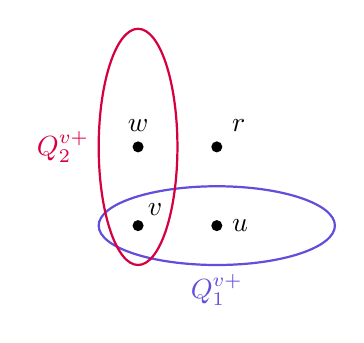
\begin{tikzpicture}
				\coordinate (O) at (0, 0);
				\fill (O) circle (2pt);
				\node[above right] at (O) {$v$};

				\coordinate (X) at (1, 0);
				\node[below = 5mm] at (X) {$\color{majorelleblue} Q^{v+}_{1}$};
				\visible<3->{
					\fill (X) circle (2pt);
					\node[right = 2pt] at (X) {$u$};
				}

				\coordinate (Y) at (0, 1);
				\node[left = 5mm] at (Y) {$\color{richcarmine} Q^{v+}_{2}$};
				\visible<3->{
					\fill (Y) circle (2pt);
					\node[above = 2pt] at (Y) {$w$};
				}

				\coordinate (r) at (1, 1);
				\fill (r) circle (2pt);
				\node[above right = 2pt] at (r) {$r$};


				\draw[majorelleblue, thick] (X) ellipse (15mm and 5mm);
				\draw[richcarmine, thick] (Y) ellipse (5mm and 15mm);
			\end{tikzpicture}
			\caption*{
				\only<1>{Let $Q^{v+}_{1}$, $Q^{v+}_{2}$ verifying the above definition.}
				\only<2>{By definition, $Q^{v+}_{1}\not\subseteq Q^{v+}_{2}$ and $Q^{v+}_{2}\not\subseteq Q^{v+}_{1}$.}
				\only<3>{Denote $u\in Q^{v+}_{1}\setminus Q^{v+}_{2}$, $w\in Q^{v+}_{2}\setminus Q^{v+}_{1}$.}
				\only<4>{As $r\not\in Q^{v+}_{1}, Q^{v+}_{2}$, both are are crossing sets.}
				\only<5>{By submodularity, if $X, Y \in {\color{atomictangerine}\mathcal{T}_{+}}$, both $X\cup{V}\in{\color{atomictangerine}\mathcal{T}_{+}}$ and $X\cap{V}\in{\color{atomictangerine}\mathcal{T}_{+}}$.}
				\only<6>{$Q^{v+}_{1}\cap Q^{v+}_{2}$ is smaller (inclusion-wise) than $Q^{v+}_{1}$ and $Q^{v+}_{2}$.}
			}
		\end{figure}
	\end{frame}

	\begin{frame}{Existence of an hyperpath that does not leave $Q^{v}_{+}$}
		\begin{tcolorbox}[colback=lightsalmon!5!white,colframe=lightsalmon!75!black,title=Lemma 12(a)]
			$\forall{s}\in V, \forall{t}\in Q^{s}_{+}$, there exists an $(s, t)$-hyperpath that does not leave $Q^{s}_{+}$.
		\end{tcolorbox}

		\begin{block}{Proof of Lemma 12 (a)}
			\begin{itemize}[<+->]
				\item By contradiction, assume that there is $s\in{V}, t\in Q^{s}_{+}$ such that any $(s, t)$-hyperpath leaves $Q^{s}_{+}$.
				\item There is $s\in Z\subseteq Q^{s}_{+}\setminus\{t\}$ such that any hyperarc leaving $Z$ will also leave $Q^{s}_{+}$.
				\item We have the following inequalities{\begin{itemize}[<+->]
					\item $d_{\vec{\mathcal{H}}}^{+}(Q^{s}_{+}) \geq d_{\vec{\mathcal{H}}}^{+}(Z)$
					\item $d_{\vec{\mathcal{H}}}^{+}(Z) \geq k$, as $\vec{\mathcal{H}}$ is $k$-hyperarc-connected.
					\item $k = d_{\vec{\mathcal{H}}}^{+}(Q^{s}_{+})$ by definition.
				\end{itemize}}
				\item We can deduce that $d_{\vec{\mathcal{H}}}^{+}(Z) = k$, which automatically implies that $Z\in{\color{atomictangerine}\mathcal{T}_{+}}$.
				\item $Q^{s}_{+}$ is not minimal, hence the contradiction.
			\end{itemize}
		\end{block}
	\end{frame}

	\begin{frame}[fragile]{Finding an admissible $(s, t)$-hyperpath in $R\in\mathcal{R}\cap{\color{caribbeangreen}\mathcal{T}_{-}}$}
		\only<1>{
			\begin{columns}
				\begin{column}{0.5\textwidth}
					\begin{figure}[H]
						\centering
						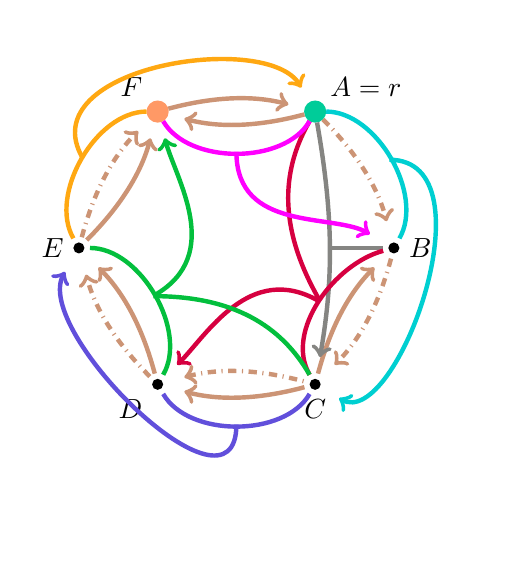
\begin{tikzpicture}
							\def\radius{2}
							\coordinate (A) at (60:\radius);
							\coordinate (B) at (0:\radius);
							\coordinate (C) at (300:\radius);
							\coordinate (D) at (240:\radius);
							\coordinate (E) at (180:\radius);
							\coordinate (F) at (120:\radius);
							
							\fill (A) circle (2pt);
								\node[above right=2pt] at (A) {$A = r$};
								\fill[caribbeangreen] (A) circle (4pt);
							
							\fill (B) circle (2pt);
								\node[right=2pt] at (B) {$B$};
	
							\fill (C) circle (2pt);
								\node[below=2pt] at (C) {$C$};
	
							\fill (D) circle (2pt);
								\node[below left=2pt] at (D) {$D$};
							
							\fill (E) circle (2pt);
								\node[left=2pt] at (E) {$E$};
	
							\fill (F) circle (2pt);
								\node[above left=2pt] at (F) {$F$};
								\fill[atomictangerine] (F) circle (4pt);
							
							\draw[ultra thick, antiquebrass, shorten <= 4pt, shorten >= 10pt, ->] (C) to [out=195, in=-15] (D);
							\draw[ultra thick, antiquebrass, shorten <= 4pt, shorten >= 10pt, ->] (F) to [out=15, in=165] (A);
							\draw[ultra thick, antiquebrass, shorten <= 4pt, shorten >= 10pt, ->] (A) to [out=195, in=-15] (F);
							\draw[ultra thick, antiquebrass, shorten <= 4pt, shorten >=10pt, ->] (C) to [out=75, in=-135] (B);	
							\draw[ultra thick, antiquebrass, shorten <= 10pt, shorten >= 4pt, <-] (F) to [out=-105, in=45] (E);
	
							\draw[ultra thick, antiquebrass, shorten <= 10pt, shorten >= 4pt, <-] (E) to [out=-45, in=105] (D);
	
							% {AC -> B}
							\draw[ultra thick, battleshipgrey, shorten <= 4pt, shorten >= 10pt, ->] (A) to [out=-80, in=80] node[pos=0.5] (ac) {} (C);
							\draw[ultra thick, battleshipgrey, shorten <= -4pt, shorten >= 4pt] (ac) to [out = 0, in = 180] (B);
	
							% TODO : Highlight @ step 18, reorient step by step (19 -> 23)
							\draw[dashdotted, ultra thick, antiquebrass, shorten <= 4pt, shorten >= 10pt, ->] (A) to [out=-45, in=105] (B);
							\draw[dashdotted, ultra thick, antiquebrass, shorten <= 4pt, shorten >= 10pt, ->] (B) to [out=-105, in=45] (C);
							\draw[dashdotted, ultra thick, antiquebrass, shorten <= 10pt, shorten >= 4pt, <-] (D) to [out=15, in=165] (C);
							\draw[dashdotted, ultra thick, antiquebrass, shorten <= 4pt, shorten >= 10pt, ->] (D) to [out=135, in=-75] (E);
							\draw[dashdotted, ultra thick, antiquebrass, shorten <= 4pt, shorten >= 10pt, ->] (E) to [out=75, in=-135] (F);
							% {AB -> C}
							\draw[ultra thick, darkturquoise, shorten <= 4pt, shorten >= 4pt] (A) to [out=0, in=60] node[pos=0.5] (ab) {} (B);
							\draw[ultra thick, darkturquoise, shorten <= -4pt, shorten >= 10pt, ->] (ab) to [out = 0, in = -30] (C);
							
							% {ABC -> D}
							\draw[ultra thick, richcarmine, shorten <= 4pt, shorten >= 4pt] (B) to [out=195, in=120] node[pos=0.5] (bc) {} (C);
							\draw[ultra thick, richcarmine, shorten <= 4pt, shorten >= -4pt] (A) to [out=-120, in=120] (bc);
							\draw[ultra thick, richcarmine, shorten <= -4pt, shorten >= 10pt, ->] (bc) to [out = 150, in = 45] (D);
							
							% {CD -> E}
							\draw[ultra thick, majorelleblue, shorten <= 4pt, shorten >= 4pt] (C) to [out=240, in=-60] node[pos=0.5] (cd) {} (D);
							\draw[ultra thick, majorelleblue, shorten <= -4pt, shorten >= 10pt, ->] (cd) to [out = -90, in = -120] (E);
							
							% {CDE -> F}
							\draw[ultra thick, darkpastelgreen, shorten <= 4pt, shorten >= 4pt] (D) to [out=60, in=0] node[pos=0.5] (de) {} (E);
							\draw[ultra thick, darkpastelgreen, shorten <= 4pt, shorten >= -4pt] (C) to [out=120, in=0] (de);
							
							\draw[ultra thick, darkpastelgreen, shorten <= -4pt, shorten >= 10pt, ->] (de) to [out = 30, in = -75] (F);
							
							% {EF -> A}
							\draw[ultra thick, darktangerine, shorten <= 4pt, shorten >= 4pt] (E) to [out=120,in=180] node[pos=0.5] (ef) {} (F);
							\draw[ultra thick, darktangerine, shorten <= -4pt, shorten >= 10pt, ->] (ef) to [out = 120, in = 120] (A);
							
							% {FA -> B}
							\draw[ultra thick, magenta, shorten <= 4pt, shorten >= 4pt] (F) to [out = -60, in = -120] node[pos=0.5] (fa) {} (A);
							\draw[ultra thick, magenta, shorten <= -4pt, shorten >= 10pt, ->] (fa) to [out = -90, in = 150] (B);
							
						\end{tikzpicture}
					\end{figure}
				\end{column}
				\hfill
				\begin{column}{0.5\textwidth}
					\begin{enumerate}
						\item Take $r$ in $V(\mathcal{H})$.
						\item Compute sets of vertices.
						\item Stopping Criteria
						\item Select a set $R$ (cf. 2.)
						\item <alert@1> Find an admissible $(s, t)$-hyperpath in $R$ to reorient
						\item Reorient the corresponding hyperpath.
						\item \texttt{Goto} (2.)
					\end{enumerate}
				\end{column}
			\end{columns}	
		}
		\only<2->{
			\begin{algorithm}[H]
				\begin{algorithmic}[1]
					\caption{Admissible $(s, t)$-hyperpath in $R\in\mathcal{R}\cap{\color{caribbeangreen}\mathcal{T}_{-}}$}
					\State{Take a set $S\in{\color{caribbeangreen}\mathcal{M}_{-}}$, with $S\subseteq{R}$, then a safe source $s\in S$.}
					\State{$Z = \{s\}$, $F = (Z, \varnothing)$, $V' = R$}
					\While{$h = (X, v)$ exists such that $v\in V' - Z$ and $X\cap Z\not=\varnothing$}
						\State Let $u\in X\cap{Z}$.
						\State $Z \leftarrow Z\cup\{v\}$
						\State $F \leftarrow F + uv$
						\If{$Q^{v}_{+}\subsetneq V'$}
							\State $V' \leftarrow Q^{v}_{+}$
						\EndIf
					\EndWhile
					\State $T = V'$
					\State Take a safe sink $t\in T$
					\State $P' = F[s, t]$
					\State $P$ is the corresponding hyperpath in $\vec{\mathcal{H}}$, obtained with $P'$.
					\State \textbf{\textsf{Return}} $S, T, s, t, P$
				\end{algorithmic}
				\label{alg_1}
			\end{algorithm}
		}
	\end{frame}

	\section{Conclusion}
	\begin{frame}{A few words about complexity}
		\begin{itemize}[<+->]
			\item We will need to transform our hypergraph as a network $(D, g)$.{\begin{itemize}
				\item The size of the network is polynomial in $|V|$ and $|\mathcal{A}|$.
			\end{itemize}}
			\item Finding an \textit{admissible} hyperpath runs in polynomial time.
			\item Computing $\mathcal{R}$, ${\color{caribbeangreen}\mathcal{M}_{-}}$, ${\color{atomictangerine}\mathcal{M}_{+}}$ in polynomial time.
			\item The number of loops in the main algorithm is polynomial.
			\item The main algorithm runs in polynomial time.
		\end{itemize}
	\end{frame}

	\begin{frame}{Conclusion}
		\only<-3>{
			\begin{alertblock}{Final words}
				\begin{itemize}[<+->]
					\item Generalization of a previous article (by \textbf{\textsf{Ito and al.}}) to hypergraphs.
					\item First efficient algorithm for computing a $k$-hyperarc-connected orientation of a hypergraph
					\item Extensions of \textsf{Main Theorem} : Starting without conditions on $\lambda(\vec{\mathcal{H}})$.
				\end{itemize}
			\end{alertblock}
		}
		
		\only<4>{
			\begin{alertblock}{Thank you for your attention.}
				\begin{figure}[H]
					\centering
					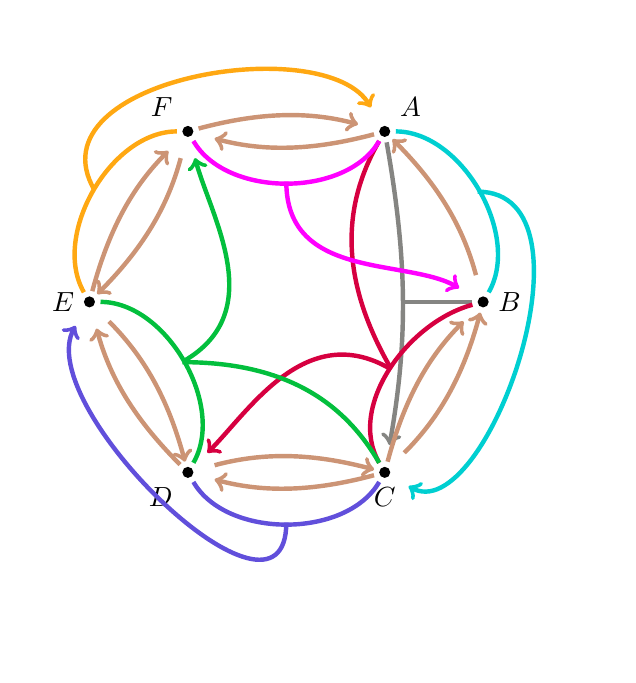
\begin{tikzpicture}
					\def\radius{2.5}
					\coordinate (A) at (60:\radius);
					\coordinate (B) at (0:\radius);
					\coordinate (C) at (300:\radius);
					\coordinate (D) at (240:\radius);
					\coordinate (E) at (180:\radius);
					\coordinate (F) at (120:\radius);
					
					\fill (A) circle (2pt); \node[above right=2pt] at (A) {$A$};
					\fill (B) circle (2pt); \node[right=2pt] at (B) {$B$};
					\fill (C) circle (2pt); \node[below=2pt] at (C) {$C$};
					\fill (D) circle (2pt); \node[below left=2pt] at (D) {$D$};
					\fill (E) circle (2pt); \node[left=2pt] at (E) {$E$};
					\fill (F) circle (2pt); \node[above left=2pt] at (F) {$F$};
				
				
					\draw[ultra thick, antiquebrass, shorten <= 4pt, shorten >= 10pt, <-] (A) to [out=-45, in=105] (B);
					\draw[ultra thick, antiquebrass, shorten <= 4pt, shorten >= 10pt, <-] (B) to [out=-105, in=45] (C);
					\draw[ultra thick, antiquebrass, shorten <= 4pt, shorten >= 10pt, ->] (C) to [out=195, in=-15] (D);
					\draw[ultra thick, antiquebrass, shorten <= 4pt, shorten >= 10pt, ->] (D) to [out=135, in=-75] (E);
					\draw[ultra thick, antiquebrass, shorten <= 4pt, shorten >= 10pt, ->] (E) to [out=75, in=-135] (F);
					\draw[ultra thick, antiquebrass, shorten <= 4pt, shorten >= 10pt, ->] (F) to [out=15, in=165] (A);
					\draw[ultra thick, antiquebrass, shorten <= 4pt, shorten >= 10pt, ->] (A) to [out=195, in=-15] (F);
				
					% {AC -> B} --> (AB -> C)
						\draw[ultra thick, battleshipgrey, shorten <= 4pt, shorten >= 10pt, ->] (A) to [out=-80, in=80] node[pos=0.5] (ac) {} (C);
						\draw[ultra thick, battleshipgrey, shorten <= -4pt, shorten >= 4pt] (ac) to [out = 0, in = 180] (B);
				
				
					\draw[ultra thick, antiquebrass, shorten <= 4pt, shorten >=10pt, ->] (C) to [out=75, in=-135] (B);
					\draw[ultra thick, antiquebrass, shorten <= 10pt, shorten >= 4pt, ->] (D) to [out=15, in=165] (C);
					\draw[ultra thick, antiquebrass, shorten <= 10pt, shorten >= 4pt, ->] (E) to [out=-45, in=105] (D); % double réorientation
					\draw[ultra thick, antiquebrass, shorten <= 10pt, shorten >= 4pt, ->] (F) to [out=-105, in=45] (E);
				
						% {AB -> C}
					\draw[ultra thick, darkturquoise, shorten <= 4pt, shorten >= 4pt] (A) to [out=0, in=60] node[pos=0.5] (ab) {} (B);
					\draw[ultra thick, darkturquoise, shorten <= -4pt, shorten >= 10pt, ->] (ab) to [out = 0, in = -30] (C);
				
						% {ABC -> D}
					\draw[ultra thick, richcarmine, shorten <= 4pt, shorten >= 4pt] (B) to [out=195, in=120] node[pos=0.5] (bc) {} (C);
					\draw[ultra thick, richcarmine, shorten <= 4pt, shorten >= -4pt] (A) to [out=-120, in=120] (bc);
					\draw[ultra thick, richcarmine, shorten <= -4pt, shorten >= 10pt, ->] (bc) to [out = 150, in = 45] (D);
				
						% {CD -> E}
					\draw[ultra thick, majorelleblue, shorten <= 4pt, shorten >= 4pt] (C) to [out=240, in=-60] node[pos=0.5] (cd) {} (D);
					\draw[ultra thick, majorelleblue, shorten <= -4pt, shorten >= 10pt, ->] (cd) to [out = -90, in = -120] (E);
				
						% {CDE -> F}
					\draw[ultra thick, darkpastelgreen, shorten <= 4pt, shorten >= 4pt] (D) to [out=60, in=0] node[pos=0.5] (de) {} (E);
					\draw[ultra thick, darkpastelgreen, shorten <= 4pt, shorten >= -4pt] (C) to [out=120, in=0] (de);
					
					\draw[ultra thick, darkpastelgreen, shorten <= -4pt, shorten >= 10pt, ->] (de) to [out = 30, in = -75] (F);
				
						% {EF -> A}
					\draw[ultra thick, darktangerine, shorten <= 4pt, shorten >= 4pt] (E) to [out=120,in=180] node[pos=0.5] (ef) {} (F);
					\draw[ultra thick, darktangerine, shorten <= -4pt, shorten >= 10pt, ->] (ef) to [out = 120, in = 120] (A);
				
						% {FA -> B}
					\draw[ultra thick, magenta, shorten <= 4pt, shorten >= 4pt] (F) to [out = -60, in = -120] node[pos=0.5] (fa) {} (A);
					\draw[ultra thick, magenta, shorten <= -4pt, shorten >= 10pt, ->] (fa) to [out = -90, in = 150] (B);
					
					\end{tikzpicture}
				\end{figure}
			\end{alertblock}
		}
	\end{frame}

\end{document}